\documentclass[twocolumn]{aastex61}
\pdfoutput=1 %for arXiv submission
\usepackage{amsmath,amstext}
\usepackage[T1]{fontenc}
\usepackage{apjfonts} 
\usepackage[figure,figure*]{hypcap}
\usepackage{multirow}
\usepackage{mathtools}
\renewcommand*{\sectionautorefname}{Section} %for \autoref
\renewcommand*{\subsectionautorefname}{Section} %for \autoref

\shorttitle{Feedback with Individual Stars}
\shortauthors{Emerick, Bryan, Mac-Low}
\newcommand{\msun}{M$_{\odot}$}
\newcommand{\ccunit}{cm$^{-3}$}

\begin{document}

\title{REDO Simulating Dwarf Galaxy Evolution with Individual Star Feedback and Chemical Evolution I: Methods and Test Case}
%Unstable Star Formation for the Lowest Mass Dwarf Galaxies
\author{Andrew Emerick}
\affiliation{Department of Astronomy, Columbia University, New York, NY, 10027, USA}
\affiliation{Department of Astrophysics, American Museum of Natural History, New York, NY, USA}
\author{Greg Bryan}
\affiliation{Department of Astronomy, Columbia University, New York, NY, 10027, USA}
\affiliation{Center for Computational Astrophysics, Flatiron Institute, 162 5th Ave, New York, NY, 10003, U.S.A}
\author{Mordecai-Mark Mac Low}
\affiliation{Department of Astrophysics, American Museum of Natural History, New York, NY, USA}
\affiliation{Department of Astronomy, Columbia University, New York, NY, 10027, USA}

%\affiliation{Institut f{\"u}r Theoretische Astrophysik, Zentrum f{\"u}r Astronomie der Universit{\"a}t Heidelberg, Heidelberg, Germany}

\begin{abstract}
\textbf{Saving this for after the first iteration}
\end{abstract}

\keywords{Galaxy -- Hydrodynamics -- Simulation -- Feedback}

\section{Introduction}

Cosmological simulations of galaxy evolution have shown increasing agreement with observations over the past decade. Recent works have been able to well capture the star forming main sequence, the stellar mass to halo mass relationship, mass metallicity relationship, etc. \citep[e.g.][]{EAGLE,Illustris1,Illustris2,FIRE,Dave2017} across a wide range of galaxy masses. On small scales, simulations have been able to resolve the long standing disagreement between $\Lambda$CDM cosmology and observed galaxies on the low-mass end without invoking new physics beyond $\Lambda$CDM. This includes the missing satellites problem \citep{Moore1999,Klypin1999}, too big to fail \citep{MBK2011,MBK2012,GK2014}, and the observed coring of inner dark matter profiles \citep[e.g.][]{Oh2011}. See both \cite{SomervilleDave2015} and \cite{NaabOstriker2016} for recent reviews on these topics. 

These simulations generally owe their successes to a combination of better accounting of the baryonic physics that governs galaxy evolution and higher resolution. In particular, a detailed accounting of both multi-channel stellar feedback processes and AGN has shown significant promise over schemes that include supernovae alone, albeit at much greater computational expense. In spite of this progress, practical considerations still limit large cosmological simulations to using sub-grid, phenomenological feedback models, often tuned to reproduce observed galaxy relationships. For this reason, we still have yet to arrive at a complete, self-consistent picture of how feedback governs galaxy evolution.

There is a considerable body of work examining the chemodynamical evolution of galaxies using cosmological hydrodynamics simulations \citep[e.g.][]{Lia2002,KawataGibson2003,Kobayashi2004,Tornatore2004,Romeo2005,OppenheimerDave2008,Wiersma2009,Shen2010,MUGS2010,ErisSimulation,Brook2014,Snaith2015,Oppenheimer2016,OWLS,EAGLE,FIRE}, nearly all of which are implemented with smooth particle hydrodynamics (SPH) schemes. Only recently have chemical evolution models been implemented in grid-based codes \citep{Few2012,Few2014,Vorobyov2015}. This is a vital and complimentary approach given the well known differences between hydrodynamics implementations \citep[e.g][]{Agertz2007,AGORA,AGORA2}. In particular, metal mixing must be handled through a sub-grid model in standard SPH schemes \citep[e.g.][]{Shen2010} that generally must be tuned to some degree to obtain reasonable results. The differences in how one handles this mixing can lead to problems in connecting the results of galactic chemical evolution models with the fundamental physics that drives the evolution \citep{Revaz2016}. We seek to produce a complementary approach to studying galactic chemical evolution with a new chemical evolution scheme implemented in the adaptive mash refinement code \texttt{Enzo} designed for high resolution simulations of isolated galaxies. 

The relative simplicity of idealized, isolated galaxy evolution simulations allows for a focused, first-principles approach to studying multi-channel feedback mechanisms. Doing so with dwarf galaxies in particular is advantageous as their small physical scales and low star formation rates allow for greater physical realism without excessive computational expense. 
We follow recent work that used low mass dwarf galaxies as laboratories to study in detail how feedback governs galaxy evolution. For example, \citet{Forbes2016} found that a self-consistent model of photoelectric heating in dwarf galaxies is an important channel of feedback. \citet{Hu2016} and \citet{Hu2017} examined the relative importance in galaxy evolution of supernovae, photoelectric heating, detailed ISM chemistry, and an approximate method for stellar ionizing radiation.

Increasing resolution, while more expensive, generally makes it easier to model physical processes in galaxy evolution. However, at high particle mass resolution ($\lesssim 10^3$ M$_{\odot}$), the standard treatment of star particles as simple stellar populations (SSP) breaks down. At these masses the IMF is no longer fully sampled, requiring a fundamentally different approach to how the simulated particles inject feedback and yields. Although there are solutions to this issue, each incurs additional model complexity with associated uncertainties. We refer the reader to \cite{Revaz2016} for a detailed accounting of this issue and possible means of addressing it. Naively, the best solution is to push towards galaxy scale simulations removing the SSP formalism and following stars individually. This allows for a detailed, star-by-star accounting of both stellar feedback and chemical enrichment without having to implement an additional sub-grid model to address the limitations of SSPs. In this work, we follow stars as individual star particles for the first time in a galaxy scale simulation.

Our work builds upon our current understanding of galactic chemodynamics while making three notable advancements: 1) direct star-by-star modeling, 2) stellar wind feedback, and 3) using an adaptive ray tracing method to follow stellar ionizing radiation. Using star-by-star modeling, we are able to capture in more detail the stellar yields from individual stars released over their lifetime. In addition to better capturing how individual metal species enrich the ISM, this allows us to chemically tag individual stars. This opens an exciting new channel for testing models of galaxy evolution by enabling us to leverage current and ongoing observations probing the detailed chemical abundances of stars in the Milky Way and Local Group. \textbf{(citations to obs campaigns - GAIA, RAVE, APOGEE, etc.).}

This paper is the first in a series of papers examining in detail the role that the individual components of multi-channel stellar feedback play in galaxy dynamical and chemical evolution. In this paper we introduce a new method of modeling for feedback physics and galactic chemical enrichment in the cosmological, hydrodynamics code \texttt{Enzo}. For the first time in galaxy-scale simulations, we model star formation down to particles representing individual stars, while simultaneously capturing stellar feedback through stellar winds, core collapse and Type 1a supernovae, photoelectric heating, and ionizing radiation through ray-tracing radiative transfer. In addition, we couple to a self-consistent set of stellar yields tables from the to track stellar yields from massive star stellar winds, AGB star winds, and supernovae. We describe each mode of our multi-channel feedback implementation in detail below, and briefly discuss their implementation in an isolated dwarf galaxy simulation.

Readers who may want to only briefly skim (or skip) over the details of our included physics are advised to just read the beginning of Section~\ref{sec:methods}, which contains a complete -- yet brief -- summary of the included physics.

\section{Methods}
\label{sec:methods}
In brief, we produce high resolution galaxy scale simulations tracking stars not as SSP's, but as individual stars sampled from an assumed IMF.
This allows us to follow star-by-star variations in feedback physics and stellar yields in detail. To properly model the ISM, we track non-equilibrium primordial chemistry (including molecular hydrogen) using \texttt{Grackle} \citep{GrackleMethod}, with heating and approximate self-shielding from a metagalactic UV background. We use updated \texttt{Cloudy} metal line cooling tables consistent with our self-shielding approximation, and an updated observationally motivated dust model for the low metallicity regimes studied here (Z $\lesssim 0.1$ Z$_{\odot}$). Each star is assigned basic properties (surface gravity, effective temperature, radius, lifetime) from tabulated stellar evolution models, which inform how the stars deposit their feedback. We directly track ionizing radiation from massive stars using an adaptive ray tracing radiative transfer method that includes the effects of radiation pressure. In addition, we follow the optically thin non-ionizing UV radiation from these stars leading to photoelectric heating and Lyman-Werner (LW) dissociation of molecular hydrogen. We track the stellar wind feedback and supernovae from these stars, depositing individual metal yields from both. We include AGB wind feedback and yields for lower mass stars, and track these directly as Type Ia supernovae progenitors. We follow yields for 12 individual metal species, chemically tagging each star with the associated local gas abundances for each species. These methods are discussed in detail below.

\subsection{Hydrodynamics and Gravity}

We use the adaptive mesh refinement (AMR) hydrodynamics and N-body code \texttt{Enzo}\footnote{http://www.enzo-project.org} to simulate the chemodyanamical evolution and detailed feedback physics in a set of high resolution, isolated, low mass dwarf galaxies. \texttt{Enzo} is an open-source code that is undergoing continual, active development by many researchers across several institutions. We use a substantially modified version of the current development version of \texttt{Enzo} (version 2.X) in this work.\footnote{This version is contained in a publicly available fork of the main repository: https://bitbucket.org/aemerick/enzo-emerick. Specifically, simulations presented here were conducted at changeset 445de816fd99.} We solve the equations of hydrodynamics using a direct-Eulerian piecewise parabolic method \citep{ColellaWoodward1984, Bryan1995} and a two-shock approximate Riemann solver with progressive fallback to more diffusive Riemann solvers in the event that higher order methods produce negative densities or energies. We compute the total gravitational potential from gas self-gravity, stars, and static background dark matter potential. The collisionless star particles are evolved with a particle-mesh N-body solver at an effective force resolution of $\sim 2 \Delta x$, where $\Delta x$ is the local cell size. 

The computational domain in an AMR simulation is adaptively refined up to a designated resolution limit for a given set of refinement criteria. We require that the Jeans length be resolved by a minimum of 8 cells, continually refining a given region until this criteria is met or the region reaches the maximum resolution. Our maximum resolution in the initial comparison simulations presented here is 2.5 pc, but our peak resolution in our fiducial set of lower mass galaxies is 1.5~pc (see Emerick et. al. in prep). At maximum resolution, the Jeans length can become under resolved, leading to artificial numerical fragmentation. Studies have shown that resolving the Jeans length by at least 4 cells is required to suppress this fragmentation \citep{Truelove1997}.

We set the star formation density threshold to the point which the Jeans length becomes resolved by only 4 cells in sub-200 K gas, or about 200 \ccunit (as discussed further in Section~\ref{sec:star formation}). Forming stars from this gas will reduce the local density, ensuring the Jeans length is resolved. However, since star formation is not instantaneous, we employ a pressure floor to support gas against artificial collapse once its Jeans length becomes unresolved. This prevents dense, self-gravitating gas from rapidly reaching densities significantly above our resolution limit.

\subsection{Chemistry and Cooling Physics}
\label{sec:chemistry}

We use the chemistry and cooling library \texttt{Grackle}\footnote{https://grackle.readthedocs.io/en/grackle-3.0/} v 3.0 to follow a nine species non-equilibrium chemistry network (H, H$^+$, He, He$^+$, He$^{++}$, e$^{-}$, H$_2$, H$^{-}$, and H$_{2}$) which includes radiative heating and cooling from these species and metals.\footnote{We use a slightly modified version of the the main \texttt{Grackle} repository, available at https://bitbucket.org/aemerick/grackle-emerick at changeset 59adc76b3130.} \texttt{Grackle} is a freely available, open source multi-code library, designed to interface with a wide variety of astrophysical codes. We outline specific model choices made in our simulations and refer the reader to \citep{GrackleMethod} for a detailed discussion of the code. We apply the \cite{Glover2008} three body rate for H$_{2}$ formation and include a model for H$_2$ formation on dust, dust heating, and dust cooling following the methods in \citet{2000ApJ...534..809O} and {2005ApJ...626..627O} as included in \texttt{Grackle}. However, we update the default dust to gas ratio scaling in \texttt{Grackle} to account for the steeper scaling in low metallicity regimes ($Z \lesssim 0.1 Z_{\odot}$) with the broken power law scalings from \cite{Remy-Ruyer2014}. For metallicities above $\sim 0.1 Z_{\odot}$, this is equivalent to the the default behavior in \texttt{Grackle}. 

Metal line cooling is modeled using pre-computed \texttt{Cloudy}\footnote{http://www.nublado.org/} tables interpolated as a function of density, temperature, and redshift, using the \cite{HM2012} UV metagalactic background. As discussed in more detail in Section~\ref{sec:diffusive heating}, we account for approximate self-shielding of H and He against this UV background. Using this prescription with metal line cooling tables computed under an optically thin assumption can lead to an order of magnitude overestimation of the cooling rate at certain densities. We use re-computed metal line tables consistent with the self-shielding approximation. Our effective cooling curve and these new tables are publicly available in the main \texttt{Grackle} repository. These are both discussed in greater detail in Appendix ~\ref{appendix:cooling}.

\subsection{Star Formation Algorithm}
\label{sec:star formation}
In order resolve individual star formation on galaxy scales, we implement a stochastic star formation algorithm adopted from \cite{Goldbaum2015,Goldbaum2016}. Each cell at the maximum refinement level is capable of forming stars if it meets the following local criteria: 1) $n_{\rm cell} > n_{\rm thresh}$, 2) $T_{\rm gas} < T_{\rm thresh}$, 3) $M_{\rm gas} > M_{\rm Jeans}$, and 4) $\vec{\nabla} \cdot \vec{v} < 0$, where $n_{\rm thresh}$ is a resolution dependent density threshold, $T_{\rm thresh}$ is a temperature threshold, and $M_{\rm Jeans}$ is the local Jeans mass. Our fiducial values for $n_{\rm thresh}$ and $T_{\rm thresh}$ are 200~cm$^{-3}$ and 200~K respectively. We limit the fraction of a cell's gas mass that is converted into stars by requiring $M_{\rm gas} > f_{\rm thresh} M_{\rm max,*}$, where $f_{\rm thresh} = 2.0 $ and $M_{\rm max,*}$ is the maximum star mass (100 M$_{\odot}$). No star formation occurs when $M_{\rm gas} < f_{\rm thresh} M_{\rm max,*}$, ensuring that a star formation episode does not produce negative densities.

We make the common ansantz that star formation occurs by converting some fraction of gas into stars in a free fall time ($\tau_{\rm ff}$) as characterized by a star formation efficiency, $\epsilon_{\rm f} \simeq 0.02$. At high resolution, one's choice of $\epsilon_{\rm f}$ is irrelevant \citep{Orr2017, FIRE2}, as star formation is ultimately self-regulated by feedback.
%but we find that $\epsilon_{\rm f}$ may impact star formation in the lowest mass halos, which are unusually sensitive to stellar ionization feedback (see Emerick et. al. in prep).
The the gas mass converted to stars in a time step, $dt$, is
\begin{equation}
M_{ {\rm gas} \to *} = \epsilon_{\rm f} M_{\rm gas} \frac{dt}{\tau_{\rm ff}}.
\end{equation}
In practice, $dt/\tau_{\rm ff} \ll 1$, and $M_{ {\rm gas} \to *}$ is smaller than the minimum star particle mass at parsec scale resolution. We therefore allow star formation to proceed stochastically, following the methods in \cite{Goldbaum2015, Goldbaum2016}, modified for variable stellar masses. In each cell that could potentially form stars, we compute the probability that 100 M$_{\odot}$ of gas will be converted into stars in that time step, and use a random number draw to determine whether or not star formation actually occurs. If it does, we random sample over the adopted IMF until 100 M$_{\odot}$ of stars form, keeping last sampled particle if the total stellar mass formed exceeds 100 M$_{\odot}$. We make the simple assumption of a Salpeter IMF \citep{Salpeter1955} with $\alpha = 2.35$, sampling over a minimum stellar mass of 1 M$_{\odot}$ and maximum stellar mass of 100 M$_{\odot}$. 

Formed stars are deposited with random positions within the star forming cell and assigned velocities equal to the cell bulk velocity with a 1~km~s$^{-1}$ velocity dispersion. Stars are assigned metallicities corresponding to the metallicity of the star forming zone, and are chemically tagged with the 14 individual species abundances (H, He, and the 12 metals) we follow in our simulations. Stars evolve throughout the simulation, losing mass from stellar winds and supernovae as described below, and by changing types, but persist throughout the entire simulation. For example, low mass stars are tagged as white dwarfs at the end of their life, which may eventually explode as a Type Ia supernova (discussed below), after which they persist as massless tracer particle ``remnants''. 

Finally, each star is marked as a ``must refine" particle, requiring that each star be surrounded by a four-cell region at the highest level of refinement. This ensures that both stellar winds and supernovae feedback are maximally resolved, and that any ejected yields are deposited over a consistent physical scale throughout the simulation.

\subsection{Stellar Properties}
\label{sec:properties}
Given their birth mass and metallicity, we interpolate over the PARSEC grid of stellar evolution tracks \citep{Bressan2012} to assign a lifetime and AGB phase start time (if any) to each star, as well as an effective temperature ($T_{\rm eff}$) and surface gravity ($g$), used in computing radiation properties (see Section \ref{sec:ionizing radiation}). We use the largest subset of the PARSEC models that are regularly sampled in our mass/metallicity space of interest, with 26 mass bins over M$_{*} \in \left[0.95, 120.0 \right] {\rm M_{\odot}}$ and 11 metallicity bins over $Z \in \left[10^{-4}, 0.017 \right]$. Although $T_{\rm eff}$ and $g$ evolve over time for stars, modifying stellar radiative properties, following a stellar evolution track for each of our stars is beyond the scope of this work. We instead fix these properties at their zero age main sequence values.

\subsection{Stellar Feedback and Chemical Yields}

\subsubsection{Stellar Yields}
\label{sec:yields}
For the first time in galaxy scale simulations, we track galactic chemodynamical evolution using stellar yields as ejected from star particles that represent individual stars. We adopt the NuGrid\footnote{http://www.nugridstars.org} collaboration's set of stellar yields given on a uniformly sampled grid in stellar mass and metallicity with 12 mass bins over $M_{*} \in \left[1.0, 25.0\right]$ M$_{\odot}$ and five metallicity bins at $Z =$ 0.02, 0.01, 0.006, 0.001, and 10$^{-4}$ \citep[][Ritter et. al. in prep]{Pignatari2016}. This grid includes yields from the AGB phase of stars between 1 and 7 M$_{\odot}$, as well as yields from both stellar winds and core collapse supernova of massive stars over 12 to 25 M$_{\odot}$. We compliment these tables to track stellar winds for stars more massive than 25 M$_{\odot}$ using tables from Slemer et. al. (in prep), based on the PARSEC stellar evolution tracks \citep{Bressan2012, Tang2014}; we ignore supernovae yields from these stars (see below). We combine all stable isotope yields for a given element into a single elemental abundance for all stable elements from hydrogen to bismuth. Although we can follow an arbitrary number of metal species, practical considerations prevent this in any given simulation. We refer the reader to previous uses of the NuGrid yields in one zone galactic chemical enrichment models \citep{Cote2016,  Cote2016_feb,Cote2017} for a detailed discussion on how various model uncertainties can influence galactic chemical evolution.

Above some mass, $M_{\rm trans}$, within the unsampled range of 7 to 12 M$_{\odot}$ stars do not undergo AGB wind phases and end their lives as core collapse supernovae. Where this transition occurs is uncertain, but is commonly taken to be around 8 - 10 M$_{\odot}$. This is a free parameter in our model, but we take $M_{\rm trans} = 8$ M$_{\odot}$ as our fiducial value. In our model, stars below this mass eject their wind yields in an AGB phase only at the end of their lives, typically over a period comparable to or less than a few time steps ($\lesssim 10$ kyr). Stars above this mass eject their stellar yields via ``massive" stellar winds at a constant mass loss rate throughout their lifetime, ending their lives as a core collapse supernova (see Section \ref{sec:stellar winds} for details on the wind energetics). Varying $M_{\rm thresh}$ changes both the time at which yields for stars around this mass are ejected (for reference, the lifetime of a 8 M$_{\odot}$ star is about 35 - 40 Myr), and the energy injection from these winds. \cite{Cote2017} explores how one's choice of $M_{\rm thresh}$ affects galaxy abundances in a one-zone model.

There are large uncertainties in stellar yields for stars more massive than 25 M$_{\odot}$ \citep[][and references therein]{Cote2016}. Indeed, even the exact fate of these stars is uncertain \citep[e.g.][]{Woosley2002,Zhang2008,Ugliano2012}, particularly as a function of metallicity \citep{Fryer2012} with potentially multiple stable/unstable regimes as a function of mass \citep{Heger2003}. Due to this uncertainty, and to avoid erroneously extrapolating from our yield tables, we adopt the simplest model and assume all stars above 25 M$_{\odot}$ end their life through direct collapse to a compact object with no mass or energy ejection.

Type Ia supernova are an important additional source of galactic chemical enrichment. These iron group rich events are responsible for the $\sim$1 Gyr timescale turnover, or ``knee", in $[\alpha/\rm{Fe}]$ vs $[\rm{Fe}/\rm{H}]$ diagrams. We use the Type Ia supernova yields given in \cite{Thielemann1986}, adopting a Type Ia supernova model as discussed in Section~\ref{sec:Type Ia}. 

\subsubsection{Stellar Winds}
\label{sec:stellar winds}
Stellar winds are important sources of early (massive stars) and late (AGB stars) enrichment and feedback in galaxies. Although the energy injected via winds over the lifetime of a cluster of stars is much less than that of supernovae and radiation, stellar winds are potentially important sources of pre-supernova feedback. In both AGB phase winds and massive star winds we inject the feedback energy in a 3-cell radius spherical region centered on the emitting star particle assuming full thermalization of the wind kinetic energy. The total injected energy in timestep $\Delta t$ is therefore $E_{\rm wind} = \dot{M}\Delta t \times v^2_{\rm wind} + E_{\rm th}$, where $E_{\rm th}$ is the thermal energy of the ejected gas mass ($\dot{M}\Delta t$) given the star's interpolated $T_{\rm eff}$. We use a monte-carlo sampling method to inject mass and energy into the surrounding cells to account for partial cell overlap at the edge if the injection region that is a result of mapping a spherical injection region to cubic grid cells.

We assume constant mass loss rates for all winds as set by the yields tables and either the lifetime of the star (for massive stars) or the length of the AGB phase (for low mass stars). 
%Properly modeling stellar winds requires sub-parsec resolution, which is problematic in galaxy-scale simulations. 
Massive star stellar winds have typical velocities on order 10$^{3}$ km s$^{-1}$ \citep{Leitherer1992}. Satisfying the Courant time step becomes prohibitively expensive following this gas ($dt \sim$~100~yr), particularly as stellar wind bubbles have typical temperatures of 2 $\times$ 10$^{6}$ K \citep{Weaver1977}. For this reason, we adopt the common simplification of reducing the wind velocity \citep[e.g][]{Offner2015}. In our case, we fix massive star stellar winds to $v_{\rm wind} = 1$~km~s$^{-1}$ for stars above 8 M$_{\odot}$. Our initial tests show that turning off energy injection from stellar winds does not significantly affect the global star formation rate of our galaxies. Due to the substantial additional computational expense of following stellar winds for Gyr timescales, we reserve examining the detailed importance of winds to future work. These points are discussed in more detail in Section \ref{sec:stellar winds discussion}.

% Injecting 10$^{3}$ km s$^{-1}$ gas onto the grid at these scales leads to super heated, shocked gas at unphysical temperatures of about 10$^{8-9}$ K, particularly when injecting into very low density media. This can lead to painfully short time step sizes and crashes in the hydrodynamics solver. We adopt the common solution of artifiially reducing the wind velocity from massive stars, choosing $v_{\rm wind} = 500$~km~s$^{-1}$ for stars above 8 M$_{\odot}$. However, this can still be problematic once the star evacuates the local ISM and injects its energy to very low density ($n \lesssim 10^{-3}$ \ccunit) gas. We address this issue by mass loading our winds when injection would lead to wind bubble temperatures in the spherical source region above a maximum temperature typical of wind bubble. This is a free parameter that we take to be 2 $\times$ 10$^{6}$ K \citep{Weaver1977}. Mass loading in this manner is (in effect) a sub-grid model for the unresolved ISM mixing at the boundary layer of the wind bubble, which is in fact the source of a majority of the gas mass within the wind bubble \citep{Weaver1977}. We take the metal species abundances of the mass loaded ISM to be the average cold / warm ISM abundance on each grid to prevent artificially inflating/deflating the overall abundances. We discuss our ability to resolve typical single star wind bubble properties in Appendix ~\ref{appendix:stellar winds}.

%parameterized in this work with the STARBURST99 wind model, \citep{Leitherer1992}:
%\begin{multline}
%{\rm log} \left[ v_{\rm wind} {\rm (km~s^{-1})} \right] = 1.23 - 0.30~{\rm log}~\left[L{\rm (L_{\odot})}\right] \\
% + 0.55~{\rm log}\left[M({\rm M_{\odot}})\right] + 0.64~{\rm log}\left[T_{\rm eff}(K)\right] \\
% + 0.13~{\rm log}\left[Z({\rm Z_{\odot}})\right].
%\end{multline}

Stars that undergo an AGB phase only deposit their feedback at the end of their lives, as determined by the PARSEC evolution tracks. AGB wind velocities vary dramatically over their relatively short lifetimes, but are typically on the order of 10 km s$^{-1}$. For simplicity, we adopt a fixed AGB phase wind velocity of 20 km s$^{-1}$ for all AGB stars.

\subsubsection{Core Collapse Supernovae}
\label{sec: core collapse}
Stars between  $M_{\rm thresh} = 8$ M$_{\odot}$ and 25 M$_{\odot}$ end their lives as core collapse supernovae, ejecting mass and yields as determined by the NuGrid stellar yield tables at 10$^{51}$ erg of thermal energy. Due to the high resolution (1.5 - 2.5 pc depending on galaxy size) of our simulations, we generally well resolve the Sedov phase of each supernova explosion (see Appendix~\ref{appendix:supernova}). We find injecting thermal energy alone in a 3 cell radius spherical region around the star particle to be sufficient to resolve the supernovae explosions. We continue to track any remaining stellar mass after the SNe as a massive ``remnant" tracer particle. In future work these particles can be used to self-consistently account for more exotic sources of feedback and chemical enrichment through X-ray binaries and neutron-star-neutron-star merger events which, while rare, could be important in long term galaxy evolution.
\textbf{Should I reference a few recent hydro sims that included these feedback sources? - AE}

\subsubsection{Type Ia Supernova}
\label{sec:Type Ia}
We continue to track low mass stars ($M < 8$ M$_{\odot}$) after their death as white dwarf (WD) particles, marking a subset as Type Ia supernova progenitors. At the end of their life, we assign a new mass to these particles following the initial to final mass relation of \cite{Salaris2009}. \textbf{I originally reproduced the equations here, but it is currently commented out. - AE}
%or, 
%\[
%M_{\rm WD} = 
%\begin{cases}
%0.134 M_{\rm i} + 0.331 & 1.7~{\rm M_{\odot}} \le M_{\rm *} \le 4~{\rm M_{\odot}} \\
%0.047 M_{\rm i} + 0.679 & 4~{\rm M_{\odot}} \le M_{\rm *}
%\end{cases}
%\]
%where $M_{\rm *}$ is the initial mass of the WD progenitor.
We follow the common assumption that progenitor stars with masses between 3 and 8 M$_{\odot}$ form WD's that are Type Ia progenitors \citep[see][ and references therein]{Cote2017}. We compute the probability that a given Type Ia progenitor will explode as a function of time using an observationally motivated delay time distribution (DTD) model. \textbf{I went in detail on the DTD model here out of frustration of the lack of detail in other works, but I can trim this if needed (AE):} The SNIa rate is taken as a power law in time, $\Psi (t) \propto t^{-\beta}$, whose slope and normalization are observables, and $\eta$ the fraction of stars which can form SN Ia progenitors that \textit{will} explode as a SN Ia within a Hubble time. The value for $\eta$ depends on the normalization of the DTD (an observable), as well as one's choice of IMF and mass range of potential SN Ia progenitors (as given above). This fraction is given as
\begin{equation}
\eta = \frac{N_{\rm Ia}}{M_{\rm SF}} \frac{\int_{M_{\rm min}}^{M_{\rm max}} m (dN/dm) dm }{\int_{M_{1}}^{M_{2}} (dN/dm) dm},
\end{equation}
where $N_{\rm Ia}/M_{\rm SF}$ is the DTD normalization, which represents the fraction of stars that form SN Ia progenitors, $M_{\rm min}$ and $M_{\rm max}$ are the lower and upper bounds of the IMF ($dN/dm$), and $M_{1}$ and $M_{2}$ are the lower and upper bounds of the range of stars that can form Type Ia candidates. The DTD slope, $\beta$, is of order unity, with typical values between 1.0 and 1.2 (see \cite{Maoz2014} for a recent review). $N_{\rm Ia}/M_{\rm SF}$ represents the number of SN Ia per mass of star formation; this can be derived by taking observed values of the SNIa rate and integrating over a Hubble time. Typical values for this are on order of 10$^{-3}$ M$_{\odot}^{-1}$ \citep{Maoz2014}. We adopt 1.2 \cite{Maoz2010} and 0.8$\times 10^{-3}$ M$_{\odot}^{-1}$ \cite{GraurMaoz2013} for our fiducial values of $\beta$ and $N_{\rm Ia}/M_{\rm SF}$. Given our choice of IMF, and with $M_{\rm min} = 1$~M$_{\odot}$, $M_{\rm max}=100$~M$_{\odot}$, $M_{1}=3$~M$_{\odot}$, and $M_{2}=8$~M$_{\odot}$, this gives $\eta = 0.041$.

Finally, the probability a Type Ia candidate will explode at a time $t$ after the formation of its main sequence progenitor is taken as

\begin{equation}
P(t) = \dot{P}(t)dt = \eta \frac{ t^{-\beta}}{ \int_{t_{\rm o}}^{t_{\rm H} + t_{\rm o}} \tau^{-\beta} d\tau} dt,
\end{equation}

where $t_{\rm o}$ is the formation time of the WD and the denominator normalizes the total probability to $\eta$. This naturally accounts for both a prompt and delayed Type Ia supernova population in our simulations.
In practice, we invert the cumulative probability distribution to assign an exact time at which a given WD will explode, rather than making a random number draw for every WD particle every time step as $\eta$ is small.

\subsubsection{Ionizing Radiation}
\label{sec:ionizing radiation}
Radiation feedback (ionization, ionization heating, and radiation pressure) is an important source of pre-SN feedback in galaxies. HII regions carved out by stellar radiation change the ISM structure where SNe eventually explode, generally increasing their dynamical importance. However, when accounting for angular effects, radiation can also allow energy from SNe to dissipate more readily through channels carved through dense clouds. Radiation feedback effects have been included with various approximations in a wide range of simulations \citep[e.g.][]{OppenheimerDave2006, Krumholz2007, HopkinsQuataertMurray2012, Agertz2013, Renaud2013, Stinson2013, Roskar2014, Ceverino2014, FIRE, AgertzKravtsov2015, Forbes2016, Hu2016, Hu2017, FIRE2}, with limited application in full radiation hydrodynamics simulations \citep{WiseAbel2012,Wise2012a,Wise2014,Kim2013a, Kim2013b,Pawlik2013,Rosdahl2015,Aubert2015,Ocvirk2016,BaczynskiGloverKlessen2015,Pawlik2017} due the additional computational expense of direct ray tracing. As we seek a complete accounting of stellar feedback physics, we follow HI and HeI ionizing radiation from our stars through ray tracing methods described below. In this particular work, we use two different simulations of the same galaxy to demonstrate the importance of following radiation feedback with full radiative transfer methods (see Section~\ref{sec:IC}). 

Enzo includes an adaptive ray tracing implementation, \textsc{Enzo+Moray} \citep{WiseAbel2011}, to solve the equations of radiative transfer as coupled to the hydrodynamics of the simulation. We follow \ion{H}{1} and \ion{He}{1} ionizing photons which are coupled to the \texttt{Grackle} primordial chemistry and heating and cooling routines to track photoionization and heating, as well as radiation pressure on hydrogen. Radiation pressure is expected to be an important source of feedback only in more massive galaxies; we explore this point further in this work.

We adopt the \ion{H}{1} and \ion{He}{1} ionizing photon rates for each star using the OSTAR2002 \citep{Lanz2003} grid of O-type stellar models, appropriate for $M_{*} \gtrsim 15$~M$_{\odot}$ at solar metallicity\footnote{The exact stellar mass range on the OSTAR2002 grid is model dependent and a function of metallicity}. We use linear interpolation in stellar effective temperature, surface gravity, and metallicity to compute the ionizing photon fluxes and rates for each star. Stars less massive than about 15 M$_{\odot}$ are generally off of the OSTAR2002 grid, and massive stars with sub-solar metallicity generally have effective temperatures above the OSTAR2002 grid. In this case, we integrate a black body spectrum at $T_{\rm eff}$ to obtain the ionizing photon fluxes, but normalize the result to be continuous with the OSTAR2002 grid (see Appendix \ref{appendix:radiation}). \citep{Dale2012} demonstrated that uncertainties on order of a few in the ionizing radiation rates are not significant in giant molecular cloud (GMC) scale simulations.
%Generally, the ionizing fluxes from high temperature black bodies underestimate the OSTAR2002 flux, and lower temperature black bodies overestimate the flux by a factor of 2-5 and 10-1000 respectively. 

Instead of assigning a fixed ionizing photon energy across all sources, we integrate over each star's blackbody curve to compute the average ionizing photon energy individually for each source (see Appendix~\ref{appendix:radiation}). The average energy for \ion{H}{1} and \ion{He}{1} ionizing photons changes significantly over the OSTAR2002 temperature range ($log(T_{4,\rm{eff}} [K]) \in \left[2.75,5.5\right]$), ranging from 15.72 eV to 20.07 eV and 26.52 eV to 31.97 eV respectively.

We also include the effects of radiation pressure on HI. This has been shown to be important in suppressing the star formation rates of dwarf galaxies by influencing turbulence and the dense gas content of the ISM \citep{WiseAbel2012,Ceverino2014}. We ignore the absorption of ionizing radiation by dust and re-radiation in the infrared. This is included in other models \citep[e.g.][]{Rosdahl2015,FIRE,FIRE2} as this may increase by a factor of a few to several the effective radiation pressure \citep{ZhangDavis2017}. However, the importance of multiple scattering is still unclear. Other works have shown the effect to only increase the radiation pressure by a factor on order of unity \citep{Krumholz2012,Krumholz2013}. Due to these uncertainties, and given that we focus on low metallicity dwarf galaxies with low dust content, we ignore this effect.

\subsubsection{Diffusive Heating}
\label{sec:diffusive heating}
We include two forms of diffusive heating in our simulations, each tied directly to the non-equilibrium primordial chemistry network in \texttt{Grackle}: 1) the optically thin, metagalactic UV background \cite{HM2012}, and 2) localized photoelectric (PE) heating from the far-ultraviolet (FUV, 6 eV $<$ $h\nu$ $<$ 13.6 eV) radiation from our stars. Photoelectric heating can be a dominant heating mechanism in the ISM \citep{Parravano2003} of the Milky Way, and could be significant in regulating star formation in dwarf galaxies \citep{Forbes2016}. However, this conclusion warrants further research as its exact importance in dwarf galaxies relative to other feedback mechanisms is contended \citep{Hu2016,Hu2017}. Generally, models for PE heating and LW radiation in hydrodynamic simulations of galaxies adopted a constant value or a static, radial profile. Only recently has the localization and time variation of these processes been considered.

Self-shielding of gas against the metagalactic UV background is important in high resolution simulations, particularly for low-mass, low metallicity dwarf galaxies where the UV background is capable of gradually photoevaporating unshielded gas from the galaxy. We have implemented the \cite{Rahmati2013} approximate self-shielding method in \texttt{Grackle} to account for HI self-shielding against the UV background (see \citep{GrackleMethod} for more details of this implementation). We assume HeI ionization generally follows HI. This allows us to approximate HeI self-shielding using the same form (A. Rahmati, private communication). We ignore HeII photoionization from the UV background entirely. Accounting for self-shielding in this manner leads to an inconsistency in using tabulated, optically-thin metal line cooling rates from Cloudy (see Section 4.1.1 of \cite{Hu2017}). As mentioned previously, we have re-computed metal line cooling tables using \texttt{Cloudy} models of optically thick clouds to be consistent with our self-shielding prescription. This is described in more detail in Appendix ~\ref{appendix:cooling}. 

%Ignoring this effect leads to an overestimation of the cooling rates when in the self-shielding regime. %We refer to \cite{2006agna.book.....O,2010MNRAS.408.1945M,2012MNRAS.421.2232F,Rahmati2013} for a more detailed description of this approximation and \cite{Gracklemethod} for its specific implementation, as used here.

We assume the FUV luminosity for each our stars is everywhere optically thin. The FUV flux in each cell is summed over contributions from each star. We parameterize the local photoelectric heating rate following \cite{BakesTielens1994}, \cite{Wolfire2003}, and \cite{Bergin2004}, where 
\begin{equation}
\label{eq:PE}
\Gamma_{\rm pe} = 1.3 \times 10^{-24} \epsilon n_{\rm H} G_{\rm eff} D \left[{\rm erg~s~cm^{-3}}\right]
\end{equation}
where $\epsilon$ is an efficiency factor that depends on $G_{\rm{o}} T^{1/2} /n_{\rm{e}}$, the attenuated local FUV flux \begin{equation} G_{\rm eff} = G_{\rm o}~\rm{exp}(-1.33\times10^{-21}~D~N_{\rm H}), \end{equation} $D$ is the dust to gas ratio, normalized to the solar value, and $G_{\rm o}$ is the local FUV flux normalized to the solar neighborhood \citep{Habing1968}. Aside from a different treatment of $D$ and the attenuation, both discussed below, this is equivalent to the method used in \cite{Hu2016} and \cite{Hu2017}.

$D$ is computed consistently with our \texttt{Grackle} dust model, using the broken power law fit from \cite{Remy-Ruyer2014} (see Section~\ref{sec:chemistry}). The extremely low dust to gas ratio in our modeled galaxies leads to a reduction in the photoelectric heating rate by approximately two orders of magnitude, as compared to a model that assumes a $D$ that scales linearly with metallicity at very low metallicity. At these low metallicities, the FUV field only becomes optically thick at length scales of $\sim$ 100 pc for densities of $n \sim 10^2$ \ccunit. Given that the ambient density of the ISM is generally 1 - 10 cm$^{-3}$, we can safely assume the FUV field to be optically thin. However, we do include a localized attenuation prescription which may influence high density or metal enriched regions of the galaxy. We approximate $N_{\rm H}$ given in the equation above locally, as $n_{\rm H}\Delta x$, where $\Delta x$ is the cell width; this approximation is necessarily resolution dependent, but substantially more computationally efficient than direct ray tracing.

Properly computing $\epsilon$ in Eq.~\ref{eq:PE} requires an accurate account of the electron number density ($n_e$). This is non-trivial in dense, neutral regions where $n_e$ is dominated by contributions from carbon, dust, and PAH ionizations; each of which are not followed directly in these simulations. Instead, we use a log-linear fit of $\epsilon$ as a function of $n_{\rm H}$ from the \cite{Wolfire2003} model of $\Gamma_{\rm{Pe}}$ in the solar neighborhood (see Figure 10b of that work); we adopt $\epsilon = 0.0148n_{\rm{H}}^{0.235}$. %This is a compromise between adoption a constant efficiency, as in \cite{Forbes2016}, and a more detailed model with more detailed non-equillibrium chemistry \cite[e.x.][]{Hu2016}.

\subsubsection{Lyman-Werner Radiation}
\label{sec:LW}
In addition to the LW radiation from the UV background, we account for localized LW flux from each of our stars to compute the total, local H$_2$ dissociation rates. Given the local LW flux, the H$_2$ dissociation rate is taken as $k_{\rm diss} = \sigma_{\rm H2} F_{\rm LW}$, where $\sigma_{\rm H2}$ is the H$_2$ dissociation cross section. We account for approximate H$_2$ self-shielding against these sources of LW flux by implementing the Sobolev-like approximation from \citet{Wolcott-Green2011} in \texttt{Grackle}. 

%
% CR section moved to missing physics
%
%\subsubsection{Cosmic Rays}
%\label{sec:cosmic rays}
%Cosmic rays may be a signficant source of feedback within star forming galaxies, capable of driving galactic outflows. Recent work has shown that CR's are capable of providing a significant additional pressure support within the ISM \citep{SalemBryan2014, SalemBryanHummels, GirichidisCR, Pakmor2016}, and are capable of producing more realistic galaxy gas halos \citep{SalemBryanCorlies}. We include cosmic rays coupled to the hydrodynamics of our simulation using a two-fluid model with adiabatic index $\gamma = 5/3$, as described in \citep{SalemBryan2014}. Cosmic ray energy is injected as some fraction, $f_{\rm CR}$, of the total supernova rate; we adopt $f_{\rm CR}$ with the fiducial value of 0.1. We include isotropic cosmic ray diffusion as described with the diffusion coefficient, $\kappa_{\rm CR} = 3.0\times10^{28}$. We refer the reader to \citep{SalemBryan2014} for a study of the effects different values for $f_{\rm CR}$, $\kappa_{\rm CR}$, and the CR adiabatic index has on galaxy evolution.

%Recent work has examined the impact anisotropic diffusion of cosmic rays along magnetic fields has on galaxy evolution \citep{GirichidisCR, Pakmor2016} and galactic winds generated from cosmic ray feedback \citep{GirichidisCR, Simpson2016}. Including magnetic fields can substantially change the effect of cosmic ray feedback provided $\mu$G level, ordered magnetic fields develop within the galaxy, as is the case for more massive disk galaxies. However, the magnetic field properties of small, ultrafaint dwarf galaxies are poorly understood. These small, puffy galaxies may be completely unable to sustain ordered magnetic fields, damping the effects of anisotropic diffusion as cosmic ray diffusion through random, tangled magnetic fields is approximately isotropic. We do not expect anisotropic diffusion and magnetic fields to have a significant impact on the effectiveness of cosmic ray feedback for ultrafaint dwarf galaxies, but this stands to be an important area of future research.

\section{Galaxy Initial Conditions}
\label{sec:IC}
The galaxy presented in this work is constructed to be similar to the observed properties of the Local Group dwarf galaxy Leo P \citep{Giovanelli2013,McQuinn2013,McQuinn2015a,McQuinn2015}, but is not intended to be a matched model to this galaxy. Leo P is gas rich ($M_{\rm gas} > M_{*}$) and low metallicity, with $M_{\rm HI} = 8.1\times 10^{5}$~M$_{\odot}$ and $M_{*} = 5.6^{+0.4}_{-1.9} \times 10^{5}$~M$_{\odot}$ \citep{McQuinn2015a} extending to a radius $r_{\rm HI} = 500$~pc, and with $12 + \rm{log(O/H)} = 7.17 \pm 0.04$ \citep{Skillman2013}, or $Z \sim 5.4\times10^{-4}$ adopting $Z_{\odot} = 0.018$ from \cite{Asplund2009}. Our dwarf galaxy is constructed without an initial background stellar population, with a total gas mass of $1.8 \times 10^{6}$~M$_{\odot}$ (or $M_{\rm HI} = 1.35 \times 10^{6}$~M$_{\odot}$) and $Z = 4.3\times 10^{-4}$, comparable to the average $z = 0$ metallicity from the stellar models computed in \citep{McQuinn2015}.

The galaxy initially consists of a smooth, exponential gas disk in hydrostatic equillibrium with a static, background dark matter potential. The gas profile follows \cite{Tonnesen2009} and \cite{Salem2015}, or
\begin{equation}
\rho_{\rm gas} (R,z) = \frac{M_{\rm gas}}{2\pi a^2_{\rm gas}b_{\rm gas}} 0.5^2{\rm sech}\left(\frac{R}{a_{\rm gas}}\right){\rm sech}\left(\frac{z}{b_{\rm gas}}\right)
\end{equation}
where $a_{\rm gas}$ and $b_{\rm gas}$ are the radial and vertical gas disk scale heights, and $M_{\rm gas}$ is approximately 70\% of the total gas mass. We set $a_{\rm gas} = 250$~pc, $b_{\rm gas} = 100$~pc, and a total gas mass of $M_{\rm T,gas} = 2.0\times 10^6$~M$_{\odot}$. We adopt a Burkert \citet{Burkert1995} dark matter potential with $M_{\rm vir} = 3.5^{8} \rm{M_{\odot}}$, $R_{\rm vir}~=~14.3$~kpc and r$_{\rm s} = 370$~pc. This gives a maximum circular velocity $V_{\rm max} = 17.4$~km~s$^{-1}$ at $R_{\rm vmax}~=~1.2$~kpc. These parameters were adopted specifically to match the observed dynamical mass of Leo P interior to 500 pc, or $M_{\rm dyn} (r < 500~\rm{pc}) = 2.7\times 10^{7}$ M$_{\odot}$, and represent virial properties near the minimum halo mass expected for galaxies of this size \citep{Ferrero2012} (need more cite). We will explore the effect of adopting different dark matter potentials within the large range of possible profiles in a future work.

Following the initialization procedure of \cite{Hu2017}, we use artificial supernova driving to generate realistic densities and turbulent properties in the galaxy ISM. This additionally prevents an otherwise uniform collapse of the gas disk. The supernovae explode at a fixed rate of $0.4$~Myr$^{-1}$, corresponding to the SFR obtained given the central HI surface density and the relation presented in \citep{Roychowdhury2009}. We stop the artificial driving 25~Myr after the first star particle forms. These artificial supernova do not drive chemical evolution of the galaxy, containing metal yields corresponding to the mean ISM abundances. 

\section{Results}
\label{sec:results}

%\begin{figure*}
%\includegraphics[width=0.23\linewidth]



%\begin{figure*}
%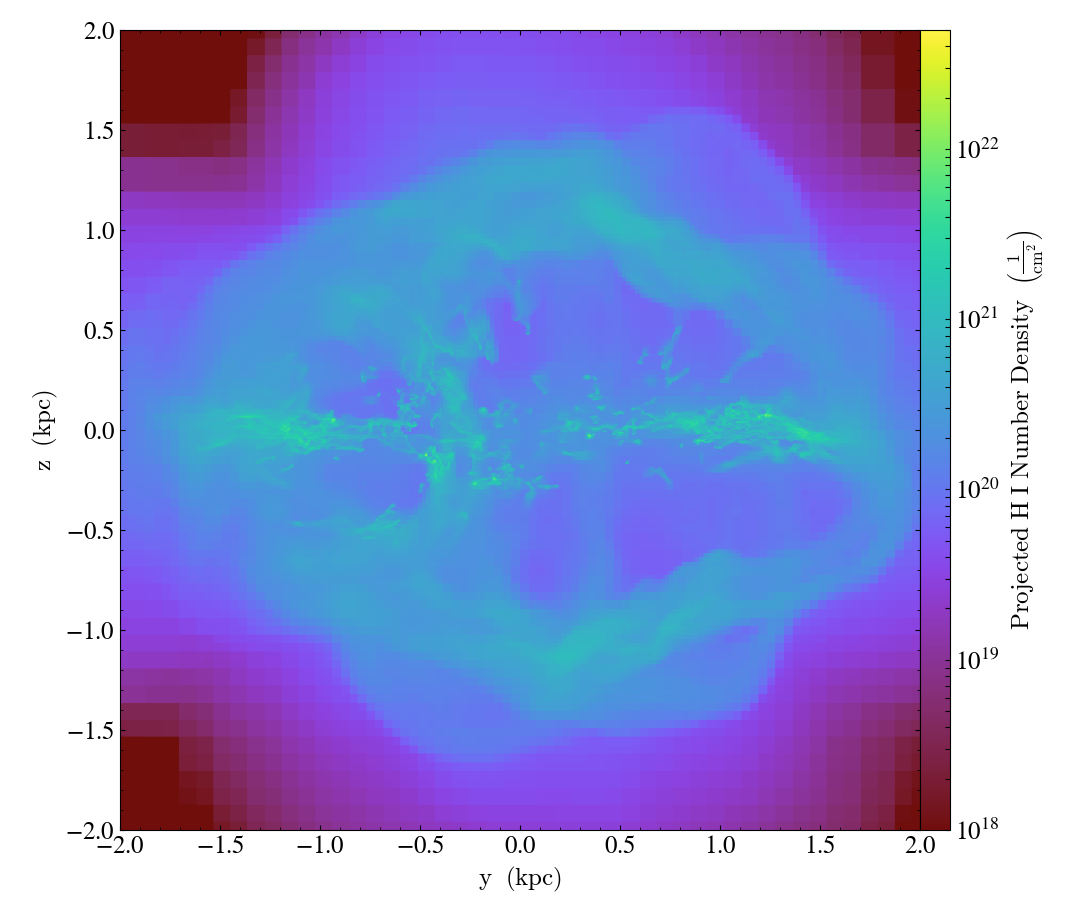
\includegraphics[width=0.23\linewidth]{panel/HI_sndriving.png}
%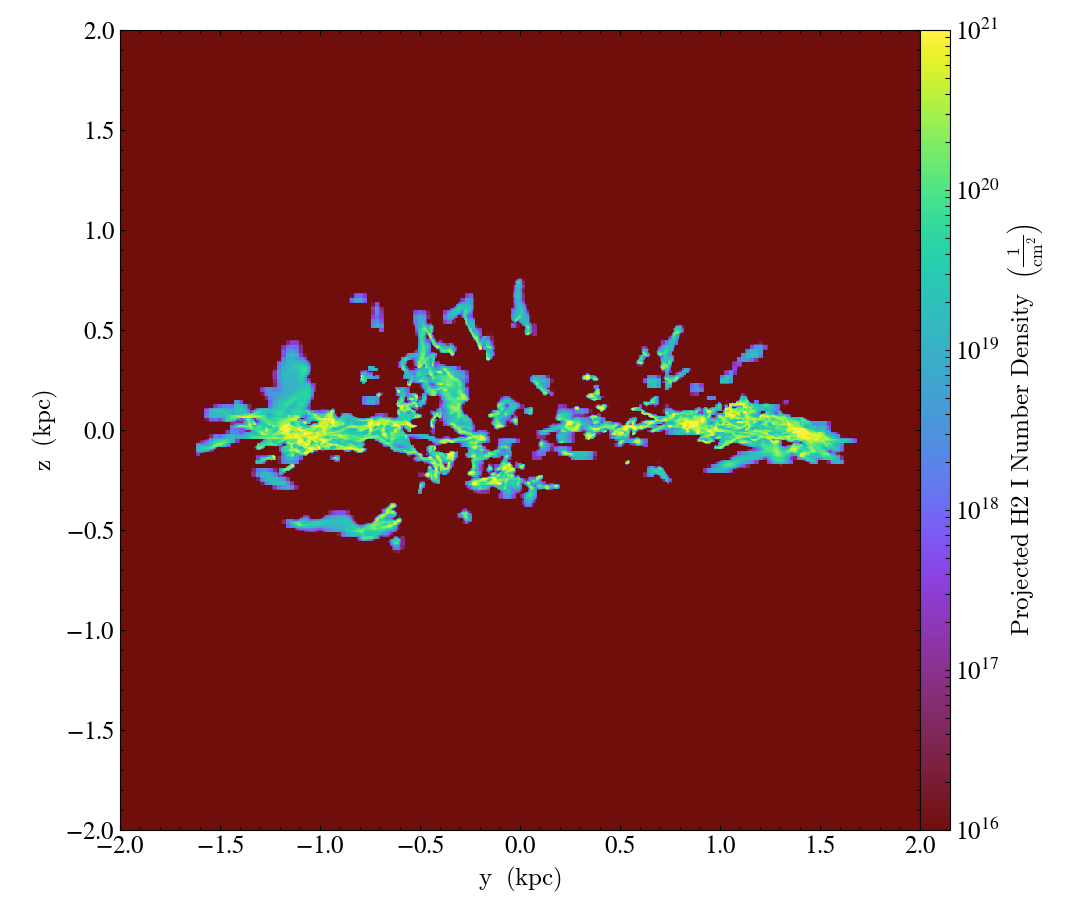
\includegraphics[width=0.23\linewidth]{panel/H2_sndriving.png}
%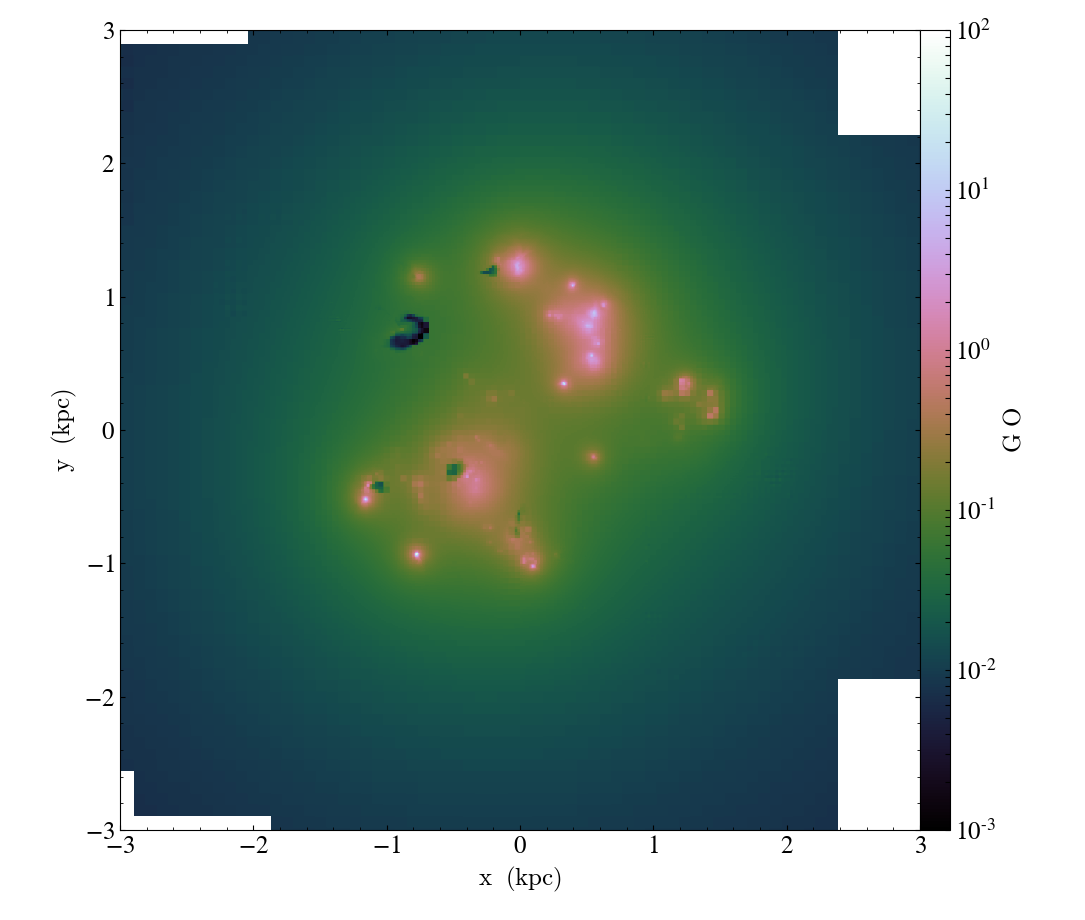
\includegraphics[width=0.23\linewidth]{panel/G_o_sndriving.png}
%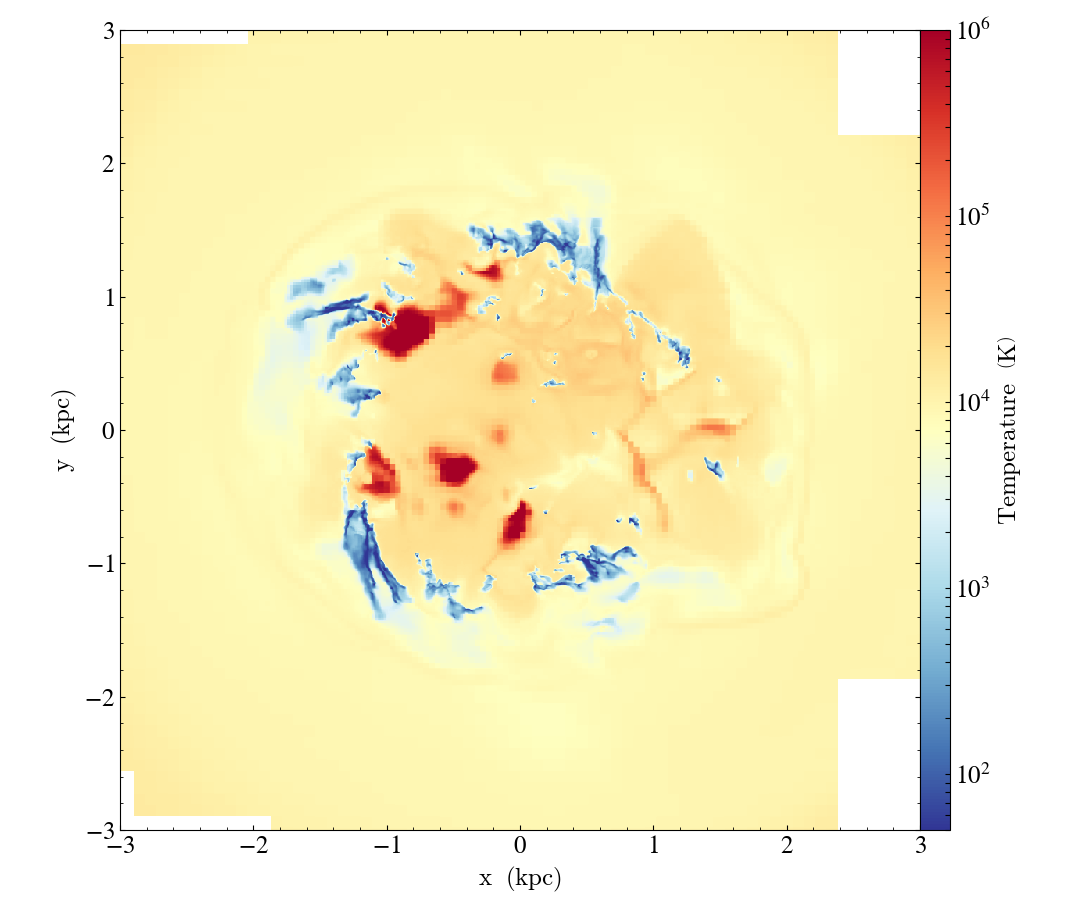
\includegraphics[width=0.23\linewidth]{panel/temperature_sndriving.png}\\
%\vspace{0.1cm}
%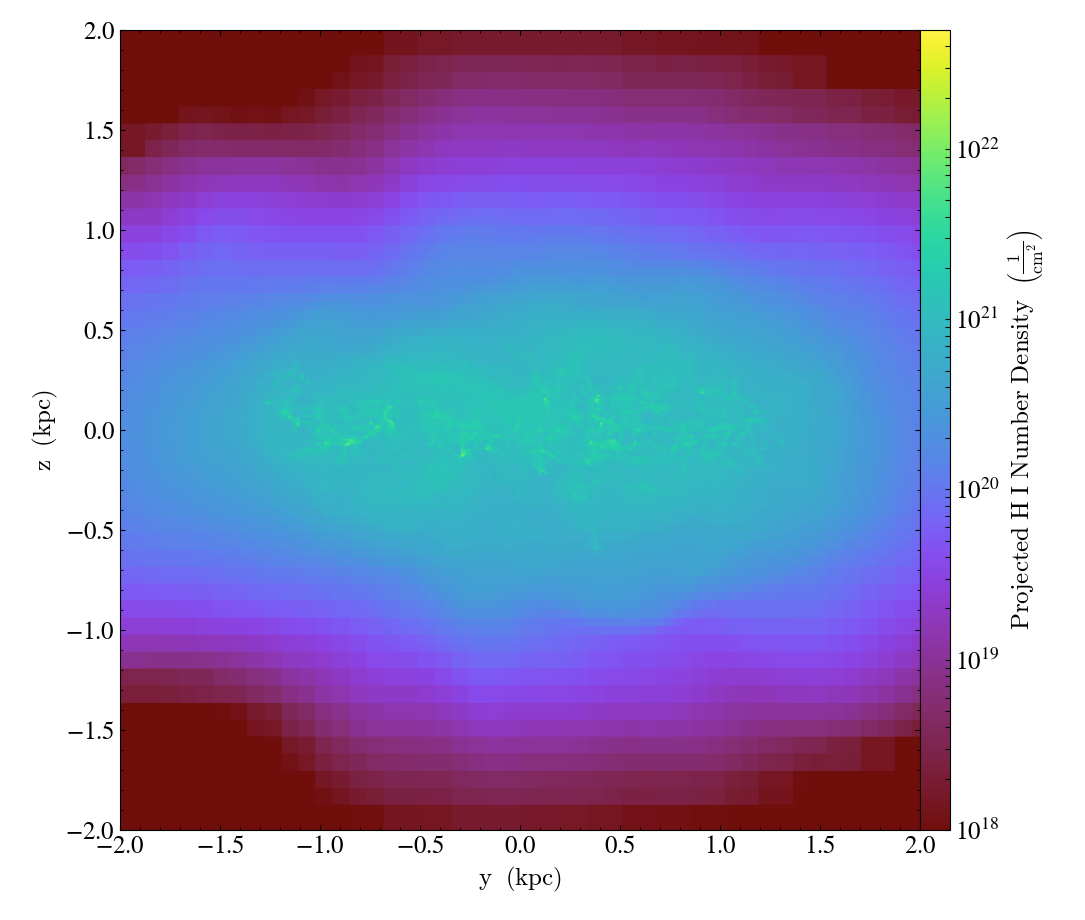
\includegraphics[width=0.23\linewidth]{panel/HI_shortrad.png}
%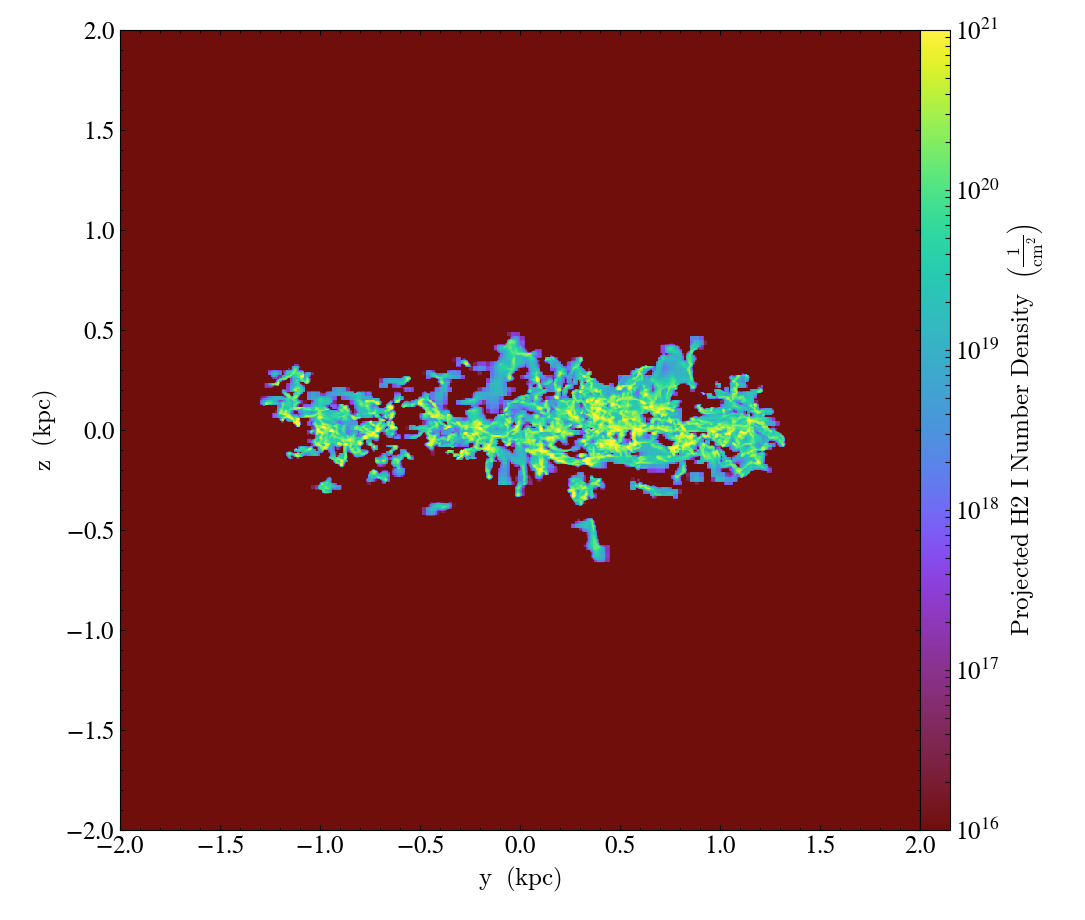
\includegraphics[width=0.23\linewidth]{panel/H2_shortrad.png}
%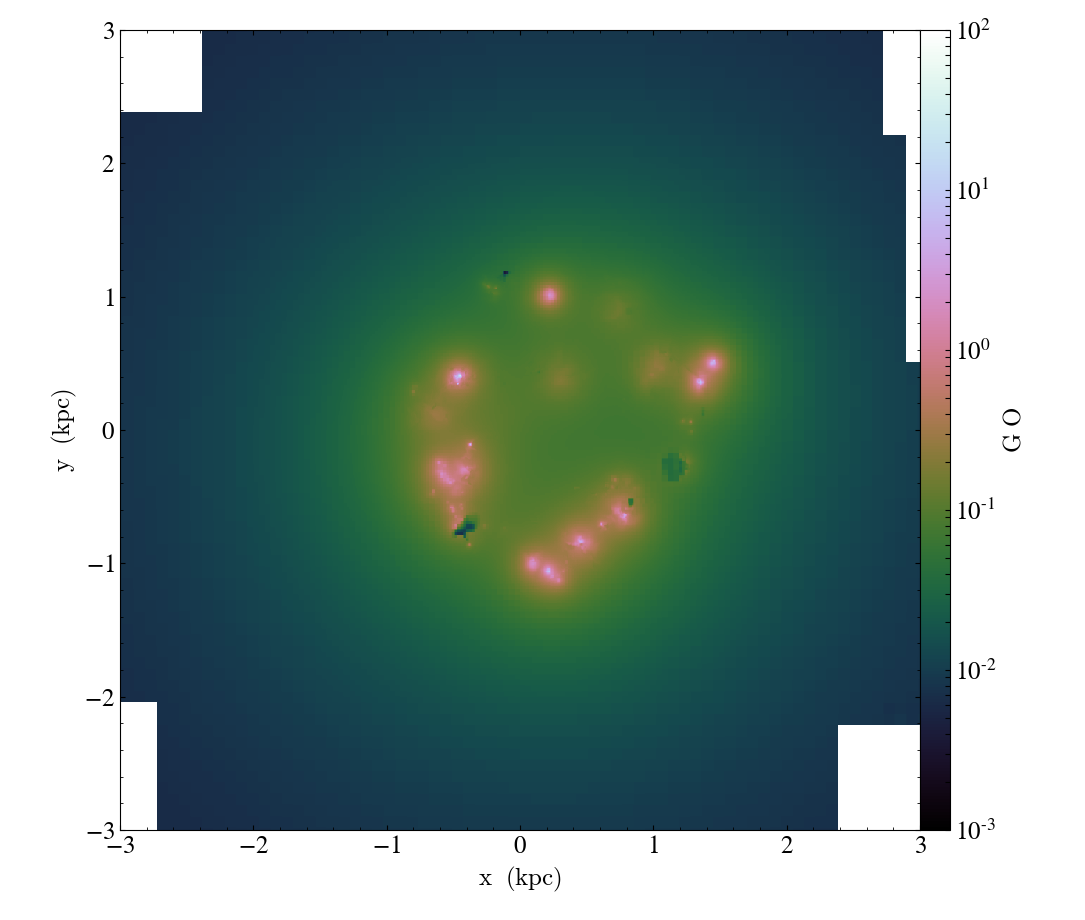
\includegraphics[width=0.23\linewidth]{panel/G_o_shortrad.png}
%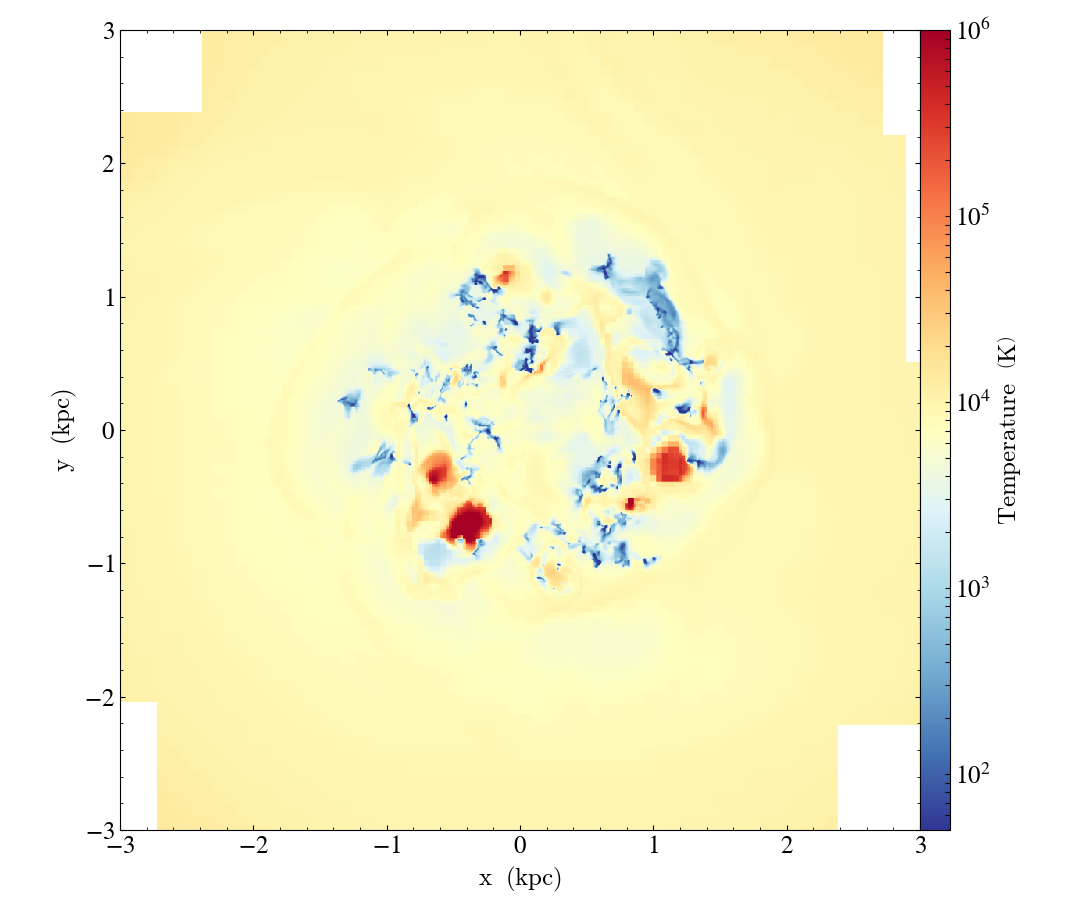
\includegraphics[width=0.23\linewidth]{panel/temperature_shortrad.png}
%\caption{Projections of our fiducial galaxy (top) and shortrad galaxy (bottom) at the end of the simulation time. The left two panels are integrated projections through the full disk, giving HI and H$_2$ column density. On the right, we show thin, face-on projections of G$_{o}$ and temperature in the central 50 pc of the disk. We note both the strange dark region in the top $G_o$ plot and the white boxes at the edges of the thin projections are artifacts of the visualization process, and are not present in the simulation.\textbf{yes plot fonts and label sizes need fixing - AE}}
%\label{fig:panel}
%\end{figure*}

\subsection{Morphological Structure}
\label{sec:structure}
We show edge-on (left) and face-on (right) projections of our fiducial galaxy (top) and shortrad (bottom) at the end of the simulation time in Figure~\ref{fig:panel}. The left two panels are number density weighted projections through the full disk, giving HI and H$_2$ column density. The right hand panels show face-on projections through thin (50 pc) slabs at the center of the galaxy for the interstellar radiation field normalized to the MW value in the solar neighborhood, or $G_o$, and gas temperature. In general, the shortrad simulation is visually consistent with that found in \citep{Hu2016,Hu2017}, exhibiting a thick, puffy disk with a relatively smooth HI column and an H$_2$ distribution that is more confined to the plane of the galaxy and is roughly uniformly distributed. Looking at the fiducial simulation, it is clear that the ray-tracing radiative transfer produces a significant change in the galactic structure. Both the HI and H$_2$ are significantly more disturbed, with notable gaps in the HI column caused by regions carved out by the ionizing radiation, and with significantly less uniform H$_2$ column, from molecular hydrogen destroyed through ionization heating. 

%\begin{figure}
%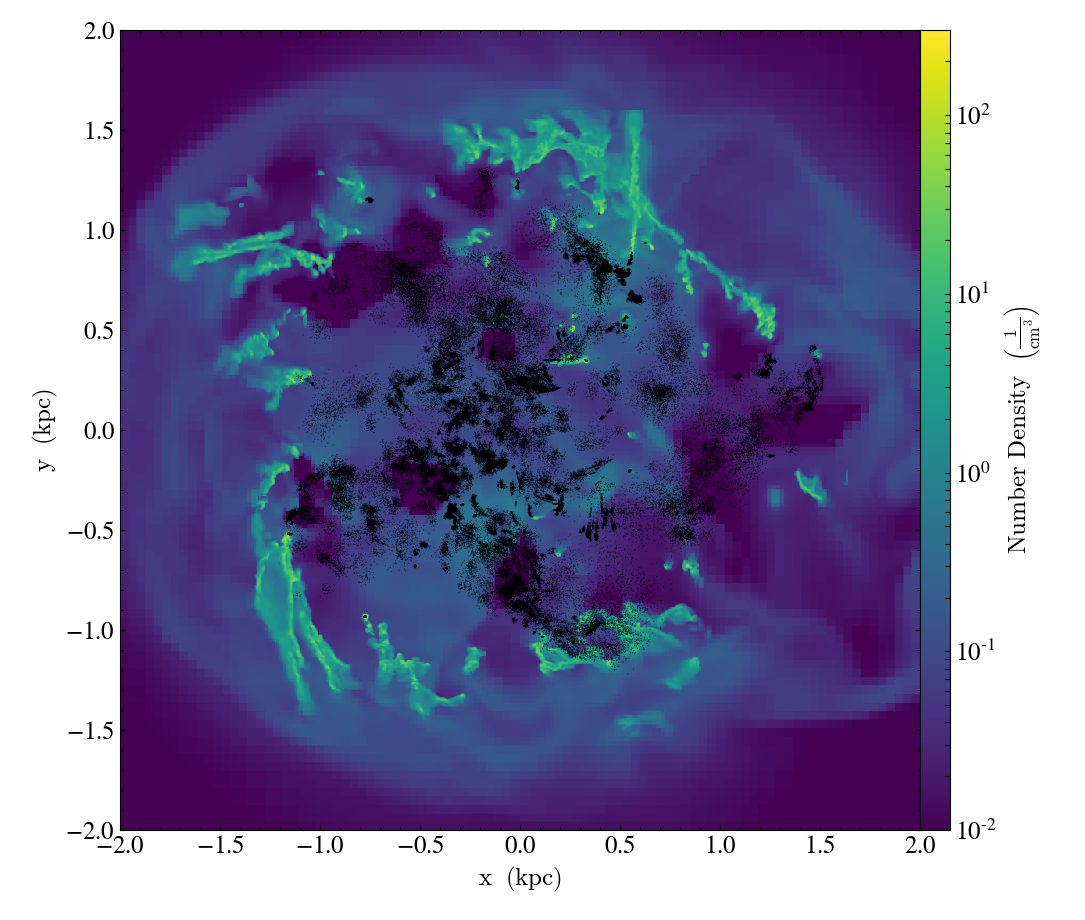
\includegraphics[width=0.9\linewidth]{panel/sndriving_particles}\\
%\vspace{0.1cm}
%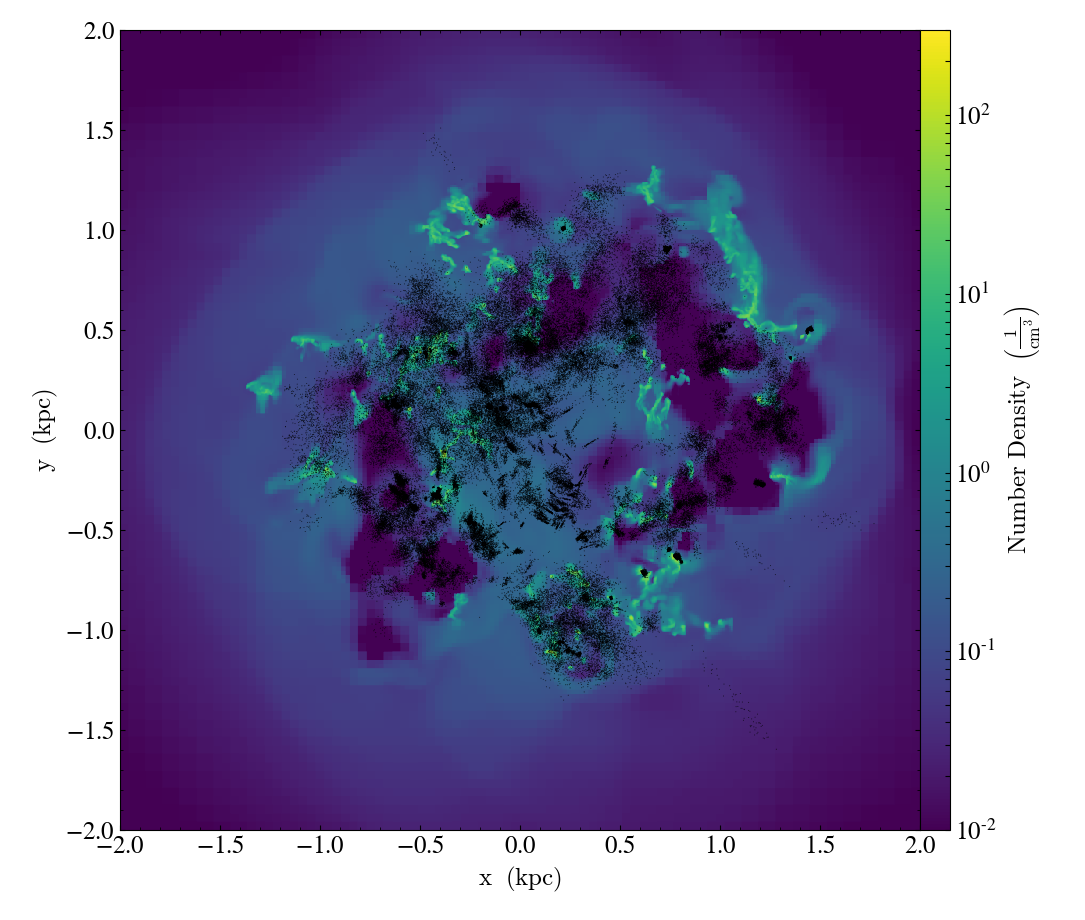
\includegraphics[width=0.9\linewidth]{panel/shortrad_particles}
%\caption{Face on, density weighted projections of gas number density for both galaxies. Each of the black points represents a single particle (star) in the simulation, and can be a living star, a white dwarf, a massless tracer originating from a Type Ia explosion, or a SNII remnant. The population is dominated by low mass stars; only a fraction of these particles have active feedback (winds, radiation, supernovae) at any one moment. \textbf{yes plot fonts and label sizes need fixing - AE}}
%\label{fig:number density}
%\end{figure}

The differences are further emphasized in the temperature projections, where a visually more significant fraction of the gas in the fiducial simulations sits at temperatures near 10$^4$~K, and much less sits at very low ($\sim$ 10 K) temperatures. The differences between gas phase in these simulations is discussed in Section~\ref{sec:phase}. The ISRF of both galaxies is quite similar, though since the ISRF in our model is generated by massive stars alone, it reflects the SFR over the previous 10 - 40 Myr, which is in fact similar in both galaxies (see Section~\ref{sec:sfr}).

Finally, in Figure~\ref{fig:number density} we present face-on projections of gas number density in both galaxies, marking each star particle in the simulation with an individual black point. Although the particles obscure some of the structure in the disk, the same general differences noted above are visible here. In particular, the fiducial simulation has significantly more disturbed gas morphology with larger regions of low density gas, and less dense gas structures.

\subsection{SFR and Mass Evolution}
\label{sec:sfr}

%\begin{figure*}
%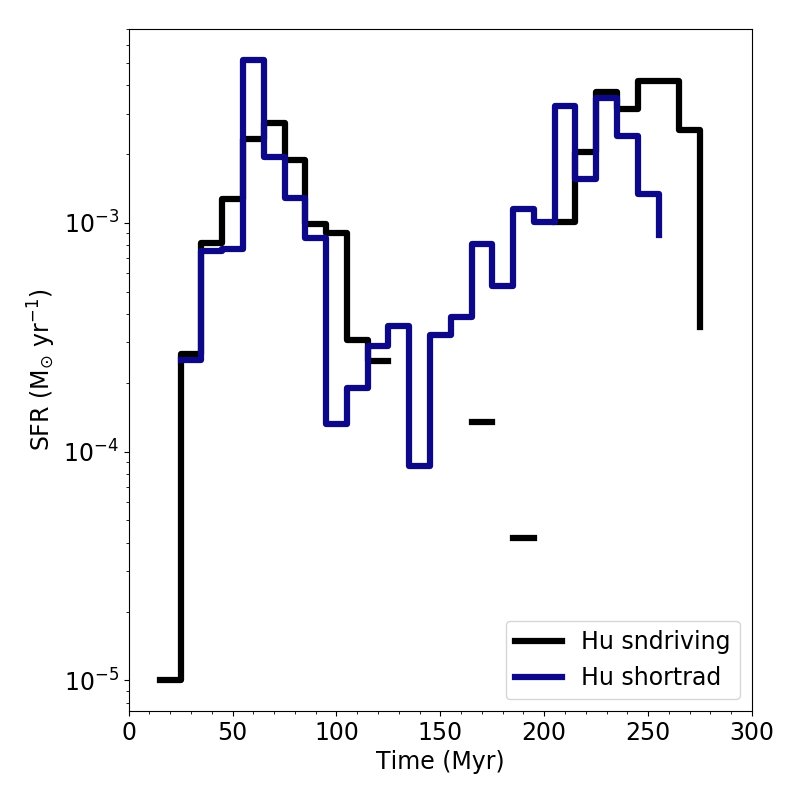
\includegraphics[width=0.32\linewidth]{sfr_comparison}
%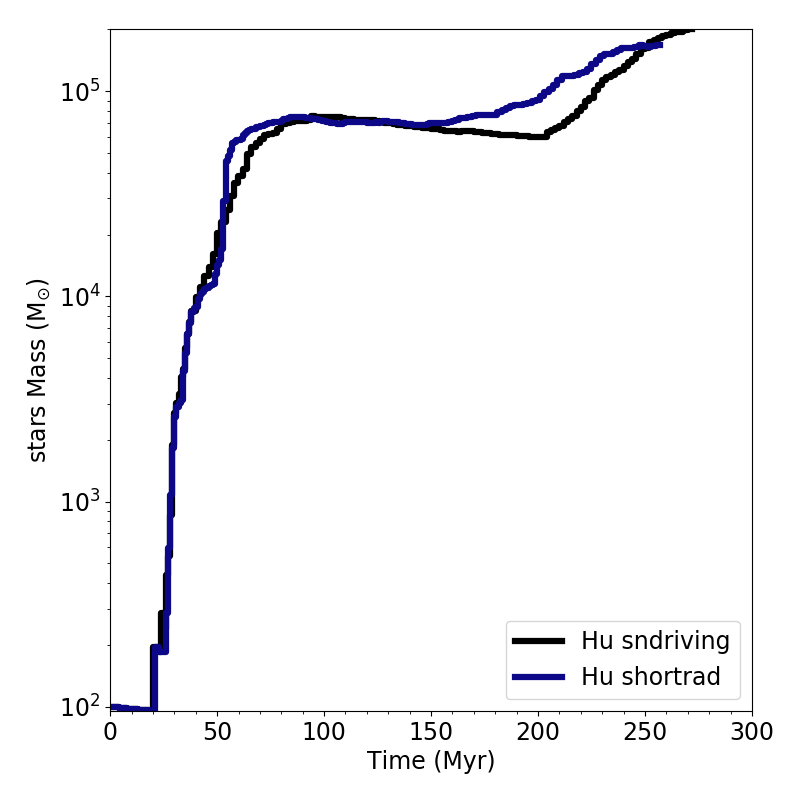
\includegraphics[width=0.32\linewidth]{stars_mass_comparison}
%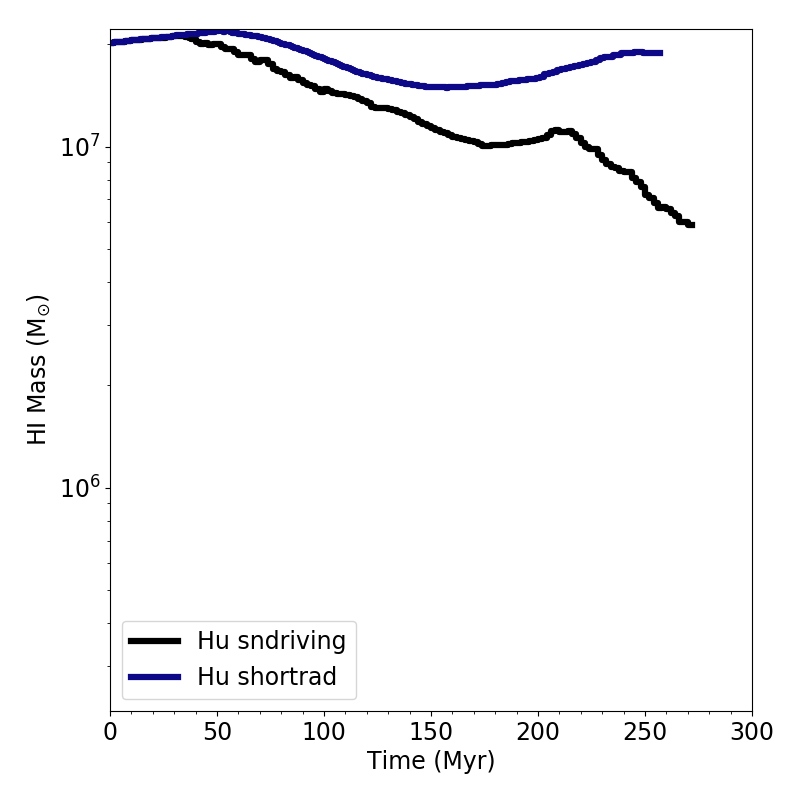
\includegraphics[width=0.32\linewidth]{HI_mass_comparison}
%\caption{The 10 Myr averaged SFR (left), stellar mass (middle), and disk HI mass (right) for each galaxy. \textbf{need to increase font sizes and y axis lim}}
%\label{fig:SFR}
%\end{figure*}

In Figure ~\ref{fig:SFR} we compare the star formation rates of both simulations (left), along with the stellar mass evolution (middle), and HI mass evolution (right). The peak and average SFRs for each galaxy over the 270~Myr simulation time are comparable, with a peak at roughly $0.04$~M$_{\odot}$~yr$^{-1}$ and an average of about $1.1~\times~10^{-3}$~M$_{\odot}$~yr$^{-1}$ in each simulation. However, the SFR evolution is qualitatively different, with the fiducial run exhibiting a $\sim$80~Myr period of minimal, patchy star formation between 125~Myr and 200~Myr ($<\rm{SFR}>~=~2.2\times~10^{-5}~$M$_{\odot}$~yr$^{-1}$). Although there is a lull in star formation during this time in the shortrad case, star formation is continuous. This difference is due solely to the long-range effects of stellar ionizing radiation, though we cannot also rule out the possibility that it also makes SN feedback more effective. It is apparent in this simulation that stellar radiation feedback is effective at suppressing star formation galaxy wide, not just locally.

%\begin{figure}
%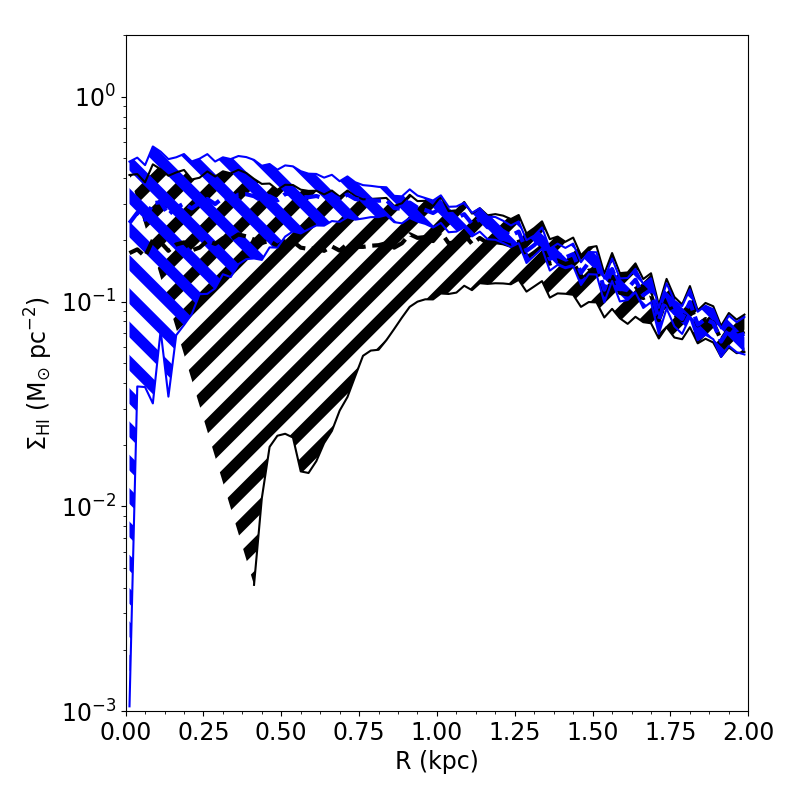
\includegraphics[width=0.9\linewidth]{HI_surface_density}
%\caption{\textbf{Coloring / style needs to change} Time averaged HI surface density profiles (dashed line) for both galaxies over the simulation time. The hatched regions show one standard deviation from the mean in each radial bin. Although there is noticeable variance in the HI profile in both galaxies, it is significantly greater for the full physics simulation. Truncating the ionizing photons to local regions alone results in a steadier and on average greater amount of HI at all but the very outer edge of the galaxy.}
%\label{fig:HI profile evolution}
%\end{figure}

The long-range effects of the ionization are clear in the HI evolution of these galaxies (middle). The presence of stellar ionizing radiation throughout the galaxy decreases the amount of HI gas present in the disk by a factor of $\sim$4, by the end of the simulation time. Figure~\ref{fig:HI profile evolution} shows the average HI surface density profile of each galaxy over the course of the simulation time, with the filled regions indicating one standard deviation from the mean. These differences in evolution lead to differences in metal production and distribution in these two galaxies, discussed further in \ref{sec:chemical evolution}.

\subsection{Outflow Properties}
\label{sec:outflows}

Show mass loading factors as a function of time here at all radii.

\begin{figure}
\centering
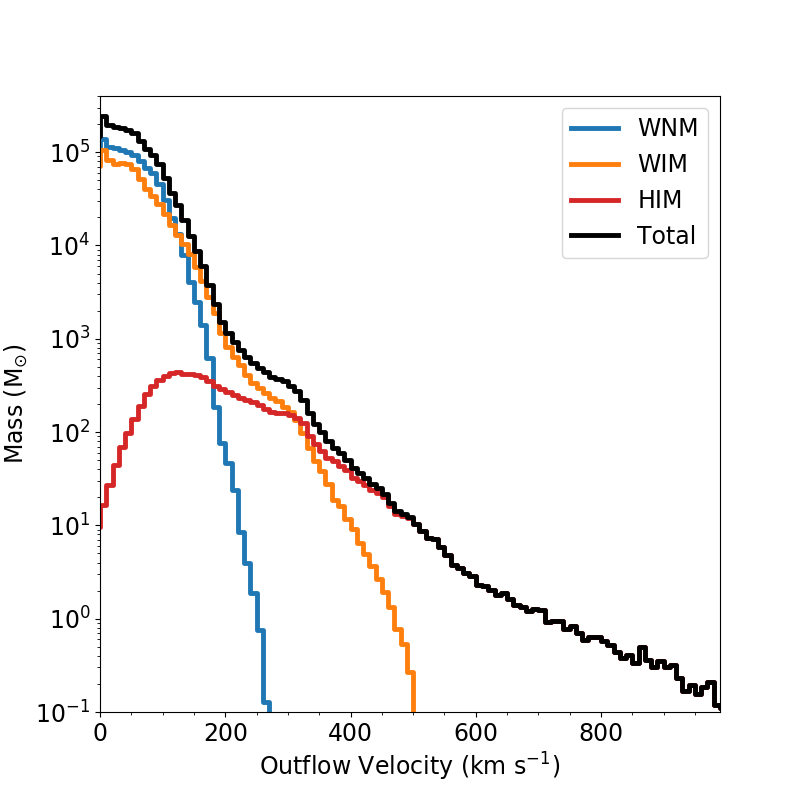
\includegraphics[width=0.95\linewidth]{outflow_velocity_distribution}
\caption{The time averaged radial velocity distribution of outflowing material external to the disk and within the virial radius of our dwarf galaxy. The outflowing material is multiphase, broken into WNM, WIM, and HIM. See XXX for definitions of these regimes. We note that WNM is often labeled simply as ``cold'', or gas below $T = 10^{4}$K. There is little to no outflowing mass in the CNM or molecular phases.}
\label{fig:outflow_velocity}
\end{figure}

Detailed outflow properties, beyond outflow rates and mass loading factors, are important discriminators between the model dependent feedback physics included in galaxy simulations. (this has been shown previously with XX XX XX producing very different outflow properties depending on what physics is included). In Figure~\ref{fig:outflow_velocity} we present radial velocity distributions of all material outside our dwarf galaxy's disk, and within the halo, broken into three gas phases. Half of the outflow, by mass, is at velocities below 40 km s$^{-1}$, with 75\% at velocities of 70 km s$^{1} or below. This gas is dominated by the two warm gas phases, with the WNM dominating at lower velocities, and the WIM at higher velocities. The distribution has a very long tail out to and beyond 500 km s$^{-1}$. These dominant launching mechanism in this simulation are supernovae (Emerick et. al. in prep), generating a rapidly moving and volume filling HIM. However, as shown the HIM comprises very little of the outflow by mass. Most of the outflowing gas comes from the warm phase, pushed out by the high pressure, fast moving HIM. Some of this warm gas certainly originates from adiabatically and radiatively cooled HIM, however. The amount of transfer between phases in the halo of our galaxy will be investigated in future work.

Final paragraph on metallicity of outflowing material.

\subsection{Phase Diagrams}
\label{sec:phase}

Our simulations contain both ample resolution and microphysics to capture a multi-phase medium within the ISM and halo of our simulated galaxy. We define five different gas phases following those defined in (Cite Draine ISM): molecular, cold neutral medium (CNM), warm neutral medium (WNM), warm ionized medium (WIM), and hot ionized medium (HIM). See Appendix (ref) for a quantitative definition of these phases. Each of these exist in our simulations, and are regulated by the complex interplay between turbulence, self-gravity, and stellar feedback throughout the galaxy's evolution. Here we discuss the phase properties of the gas throughout the simulation box and within the ISM of our dwarf galaxy.

Figure~\ref{fig:phase} shows the temperature-density phase diagram of all gas in the simulation domain, averaged over the final 50 Myr of simulation time. One can readily identify the two most massive regions of gas in the simulation, a low density, warm phase produced through ionization and supernovae heating, and a cold, high density phase which makes up most of the mass in the galaxy's disk (see Figure~\ref{fig:ISM_evolution}). [discuss what is / is not in disk from this diagram]

\begin{figure*}
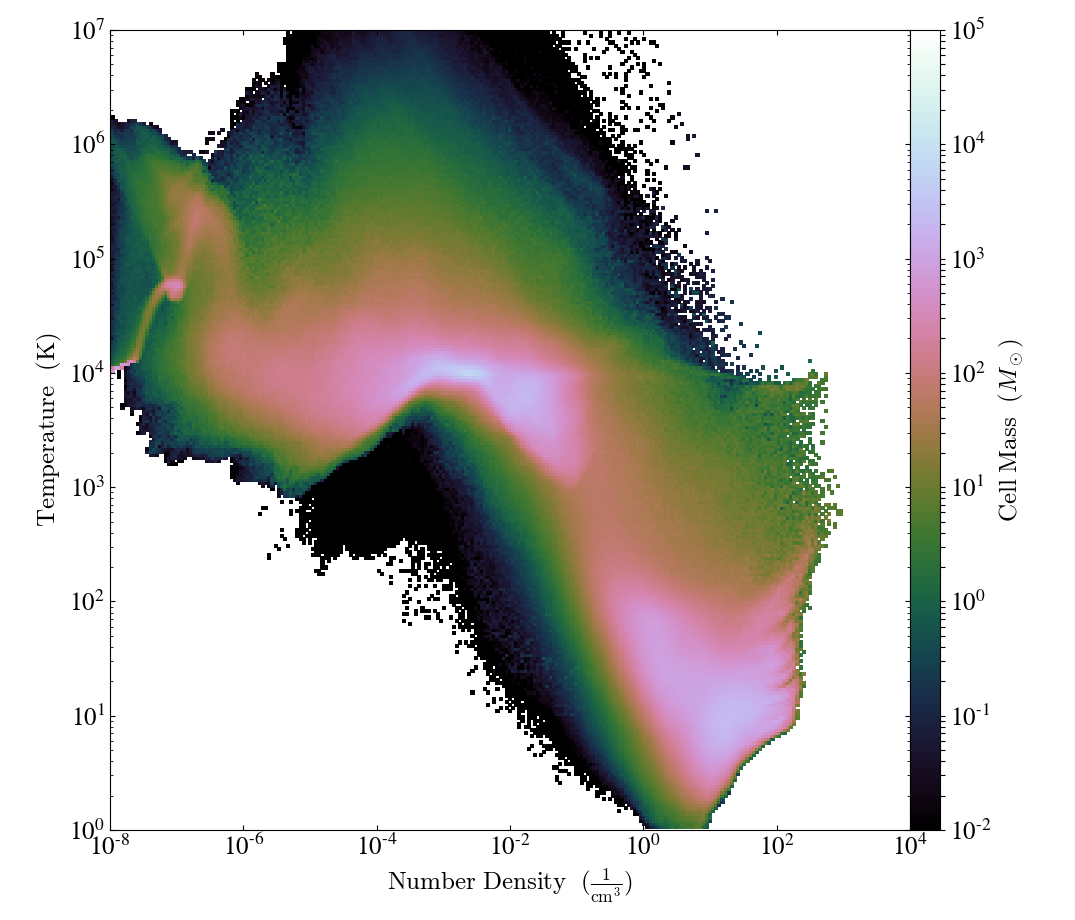
\includegraphics[width=0.45\linewidth]{phase_diagram.png}
\caption{The full-box temperature vs. number density phase diagram of our dwarf galaxy simulation, averaged over the final 50 Myr of simulation time.}
\label{fig:phase}
\end{figure*}

The mass of the ISM in our dwarf galaxy is dominated by the CNM over the entire simulation time, as shown in the left panel of Figure~\ref{fig:ISM_evolution}. Together, the CNM and WNM comprise roughly 90\% of the galaxy's gas mass. The hotter WIM and HIM contain little mass, but by far dominate the ISM volume, as shown in the right panel. (more here)

\begin{figure*}
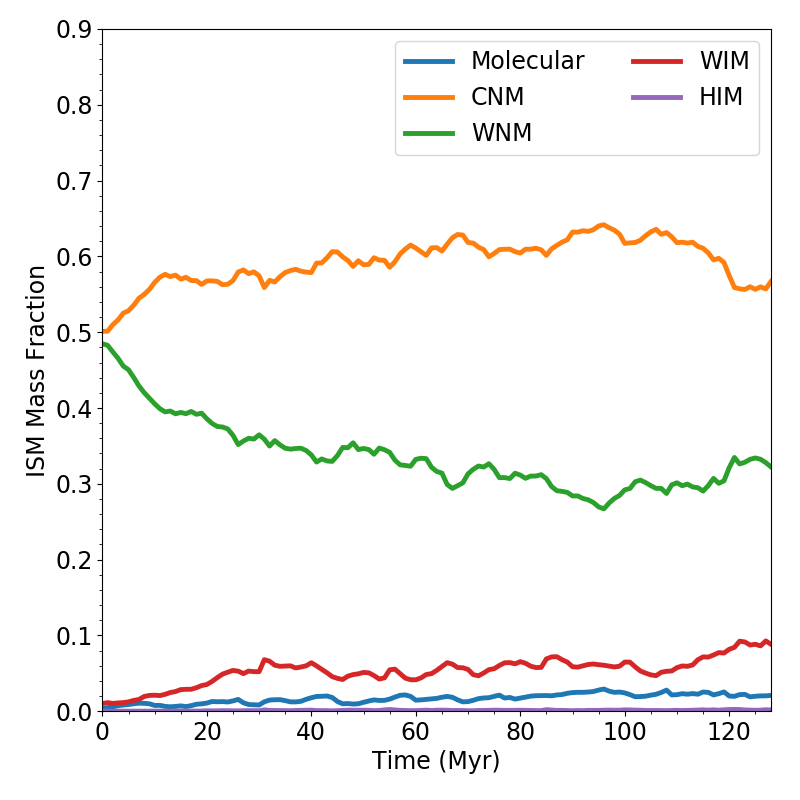
\includegraphics[width=0.45\linewidth]{mass_fraction_evolution.png}
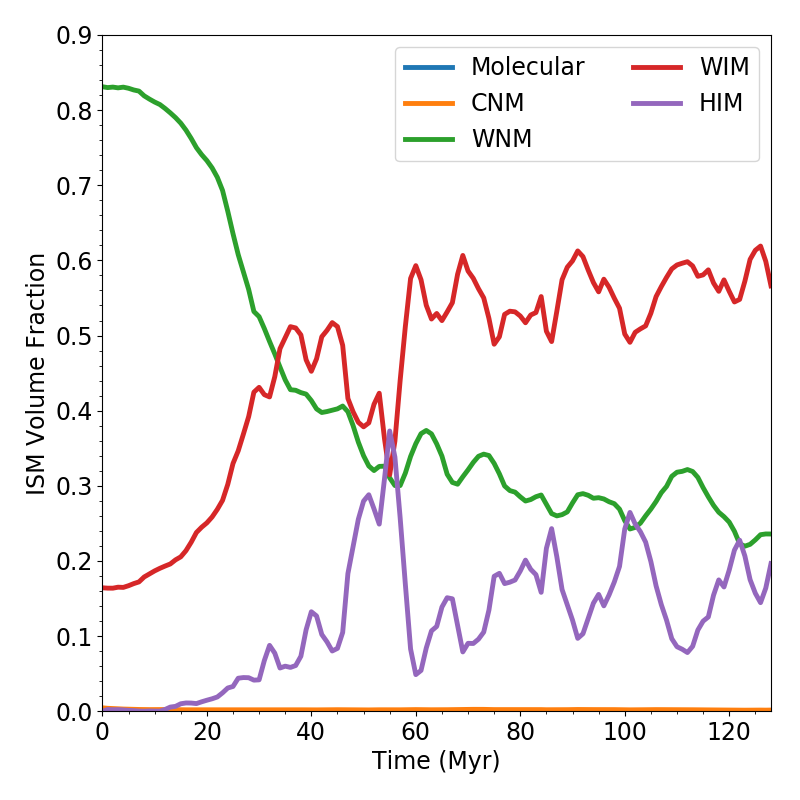
\includegraphics[width=0.45\linewidth]{volume_fraction_evolution.png}
\caption{The evolution of the mass and volume fractions for each phase of our galaxy's ISM. This figures only consider gas present within the disk of the galaxy.}
\label{fig:ISM_evolution}
\end{figure*}

\subsection{Chemical Evolution} %and Metal Enriched Outflows}
\label{sec:chemical evolution}
Although our simulations are long enough to begin to discuss morphological and dynamical differences between the galaxies, they are too short to focus in detail in chemodynamical evolution. For this reason, we make only a brief comparison between these two galaxies, saving a more detailed examination for our simulations of lower mass dwarf galaxies run for $\sim$Gyr timescales (Emerick et. al. in prep).

%\begin{figure}
%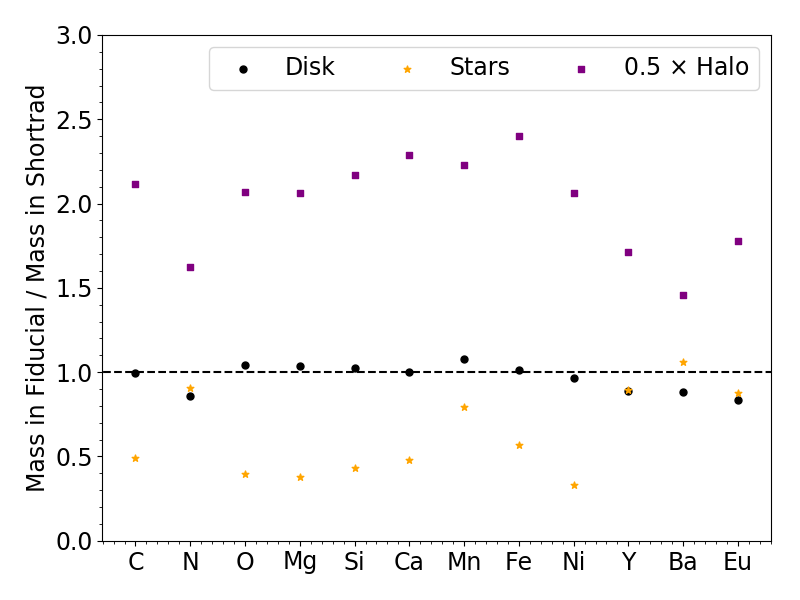
\includegraphics[width=0.9\linewidth]{element_mass_comparison_fraction}
%\caption{Ratio of amount of mass in a given mutually exclusive phase (disk, halo, and stars) between the fiducial and shortrad simulations. The halo ratio has been multiplied by 0.5 for clarity. We caution against making any interpretation of Mn and ratios for the s and r-process elements (Y, Ba, and Eu) as there is very little mass of these elements produced in the $\sim$100 Myr timescales examined here. \textbf{comment: I thought of a few different ways of conveying this information, but all were painful to look at or make (e.x. double bar graph showing fractional element dist)... this was the least painful, but open to suggestions}.}
%\label{fig:element mass ratio}
%\end{figure}

In Figure~\ref{fig:element mass ratio} we divide the total mass of each element contained in each of three regimes (stars, disk, or halo) of the fiducial simulation by the mass in the shortrad simulation (i.e. $>$ 1 means more mass in the given in the given phase in the fiducial simulation). We multiply the halo ratio, defined as all elements outside the disk but within the virial radius, by 0.5 for clarity. Although the total metal production in each galaxy is similar, the partitioning of those metals differs significantly.

The fiducial simulation contains more (by a factor of 3 to 5) mass in a given species in the halo than the shortrad simulation. The additional feedback produced by tracing radiation outside 50 pc from each stars effectively drives gas and metals out of the disk. Most of this gas driven into the halo is still contained well within R$_{\rm vir}$ of this galaxy. It is unclear whether or not the additional feedback in the fiducial model will be able to move gas farther out into the halo. We note that a majority of the produced mass is still in the disk for each simulation, which is why the disk ratios are around unity. Though it varies for each element, the halo masses represent 10-20\% of the disk mass for the fiducial simulation, and 3-5\% for the shortrad simulation. 

The feedback differences also impact the stellar metal abundance evolution in each galaxy. On average, the total mass of each element locked away in stars in the shortrad simulation is roughly twice as much as that contained in stars in the fiducial simulation. This is somewhat surprising because not only does the fiducial simulation have a slightly greater stellar mass by the end of the 270 Myr run time (2 $\times$ 10$^4$ M$_{\odot}$), but it also forms more of its stars later than the shortrad simulation. Naively, this should mean there would be more mass in a given element locked in the fiducial simulation stars as it has both more mass in stars and there has been slightly more time for produced metals to mix with the ISM and into these stars. This implies that differences in feedback evolution can lead to potentially significant differences in stellar abundances.

We caution against any interpretation of the ratio for Mn and the ratios for the s-process and r-process elements (Y, Ba, and Eu) as there is very little mass in these species in either simulation. However, we do point out that the ratios for N are qualitatively different than each other element. There is more N in the shortrad disk than the fullrad and its ratios are all much closer to unity than any other element. We suspect this is because, at these low metallicities, the IMF weighted N production is dominated by stellar winds of massive stars around $8 - 10$~M$_{\odot}$ and AGB stars\footnote{Although AGB stars are less relevant on these timescales. The lifetime of a 5 M$_{\odot}$ star at these metallicities is on order of 100 Myr} . However, IMF weighted production for the other species are dominated by SNe. This means most of the N produced is injected in a wind phase. This is more easily retained and mixed in the ISM than the other elements which are injected with much higher energy in SNe. These initial results immediately suggest that differences in both included feedback and mechanisms for yield injection can create discernible differences in stellar abundance patterns. How abundance variations like this evolve over longer timescales in lower mass dwarf galaxies is the subject of ongoing work (Emerick et. al. in prep.). 

\textbf{I did have a panel plot showing column for each element here, but decided to take it out. Might be worth putting in panel comparison for a few elements, but not sure. Suggestions? - AE}
%\begin{figure*}
%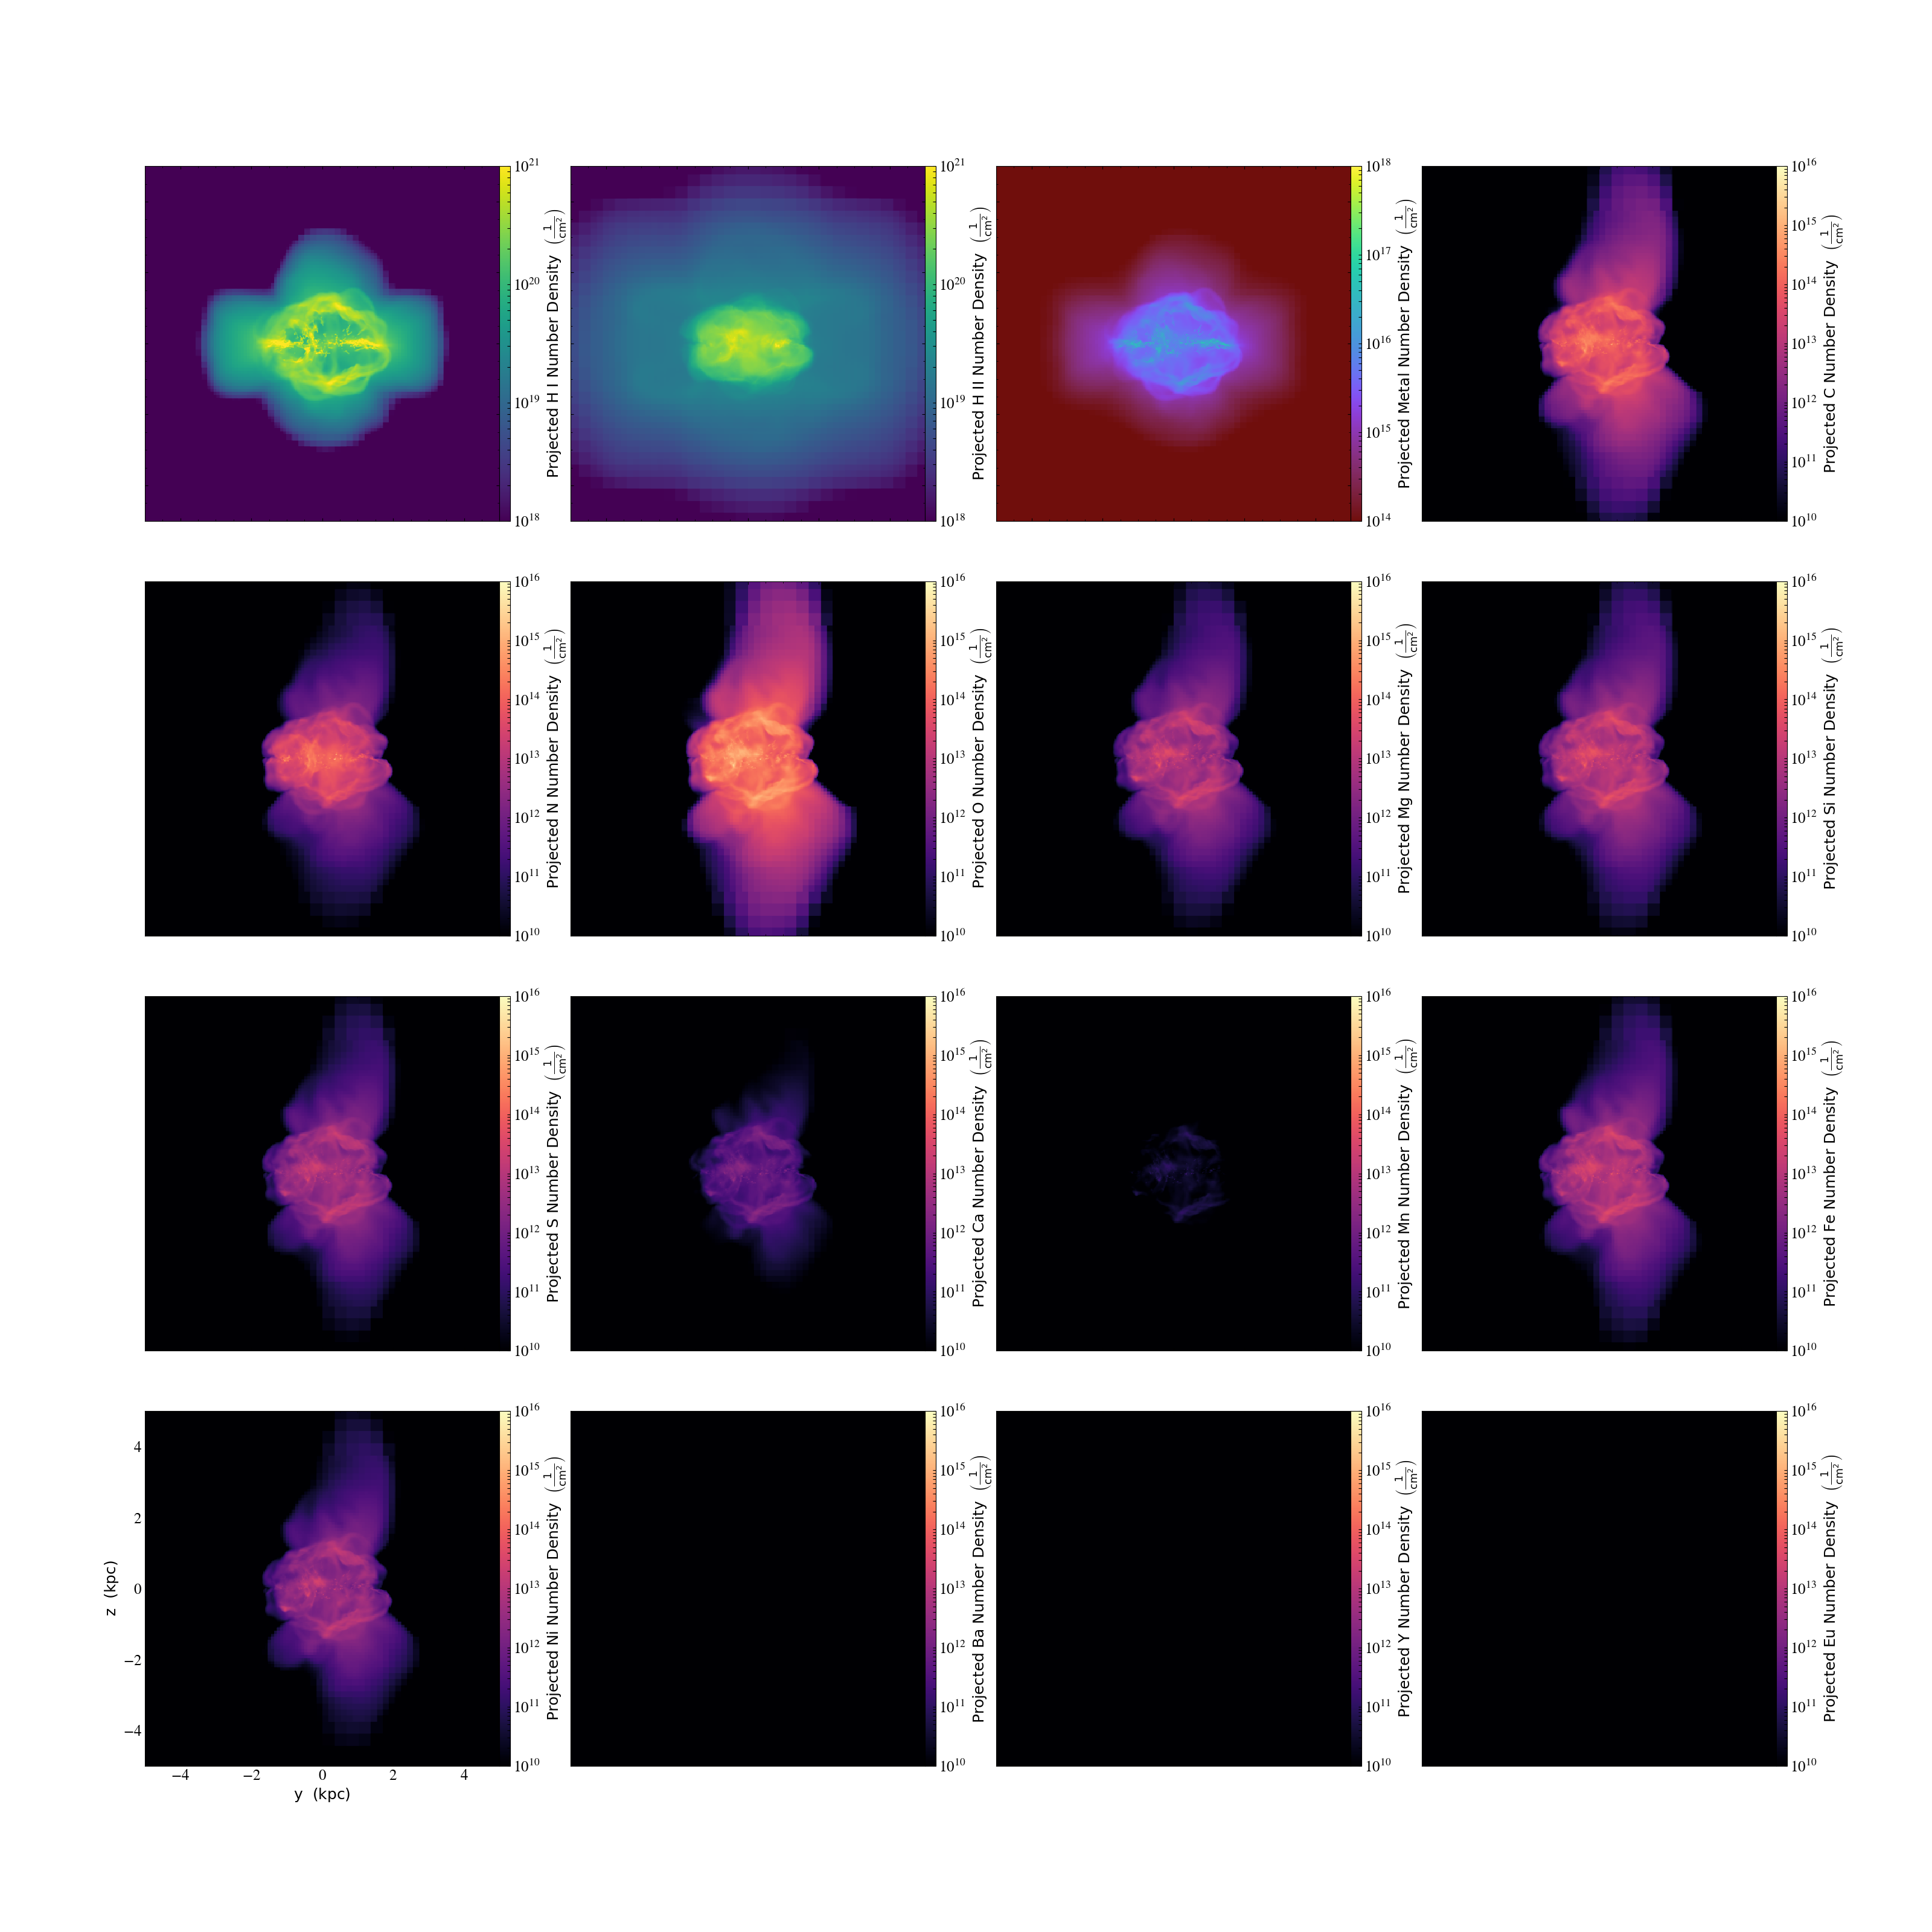
\includegraphics[width=0.9\linewidth]{DD0204_elements}
%\caption{Panel plot of elements \textbf{PLACEHOLDER FOR NOW}}
%\label{fig:elements panel}
%\end{figure*}

\section{Discussion}
\label{sec:discussion}

\subsection{Comparison to Previous Work}
\textbf{I am going back and forth on how much this is needed given the above comparison to Hu's simulations. Thoughts? - AE}
% still not sure what to do here... 

\subsection{Missing Physics}
Although we include detailed physics in our simulations, there remains additional physics that may be relevant.These are discussed below.

\subsubsection{Full Stellar Wind Model}
\label{sec:stellar winds discussion}
As discussed previously, our stellar wind model significantly reduces the injected wind velocity from $\sim$1000 km s$^{-1}$ to 1 km s$^{-1}$. Although our model is capable of generating realistic stellar winds with temperature profiles and radial evolution comparable to those expected from analytic calculations \citep{Weaver1977}, the hot, fast winds place a near constant and severe constraint on the Courant time step that renders $\gtrsim$100~Myr simulations impractical. When considered in isolation, stellar winds are an important source of pre-SN feedback and do dramatically influence the dynamical evolution on molecular cloud and galaxy scales \citep{Dale2008,Peters2017,Gatto2017}. However, when considered together with ionizing radiation, stellar winds contain less total energy \citep{Agertz2013} and do not seem to have a significant dynamical influence in either idealized simulations \citep{Geen2015} or GMCs \citep{Dale2014}. They are even less relevant in the low-metallicity regime studied here, as stellar winds become weaker with decreasing metallicity \citep{Puls2000, Vink2005}. Although they likely have no dynamical importance, a full model of stellar winds may affect detailed ISM properties and metal mixing, warranting a closer examination in a future work.

%old comment: (need to ref or back up this claim: see Dale et al. 2014 for individual clouds, while the right panel of Fig 2 in Shull \& Saken 1995 shows that the integrated wind energy from a cluster is about 10\% that of the supernovae -M). 

\subsubsection{Cosmic Rays and Magnetic Fields}
Recent work has explored the importance of cosmic ray feedback in regulating the ISM and wind properties in galactic disks \citep{Hanasz2013,GirichidisCR,Simpson2016,Farber2017} and simulations of both isolated \citep{SalemBryanCorlies,Salem2015,Pakmor2016,Ruszkowski2017} and cosmological galaxies \citep{SalemBryanHummels}. These relativistic charged particles act as a source of non-thermal pressure support in the galaxy's ISM, capable of driving outflows with different phases and velocities than those driven through stellar feedback alone \citep{SalemBryanCorlies}. Modeling cosmic rays is challenging, however, as they encompass a wide range of energies (give range), with significant uncertainties in how they propagate through the ISM \citep[e.g.][]{Wiener2017}. Their propagation is often modeled as a diffusive process, but in truth this diffusion should vary depending on cosmic ray energy. In addition, cosmic rays couple effectively to the magnetic fields of galaxies, diffusing preferentially along structured magnetic field lines within the ISM. Modeling cosmic ray feedback completely requires both an accurate cosmic ray model and magnetohydrodynamics in order to capture the interplay of these two physical phenomena. Finally, including MHD presents additional difficulties in untangling the effects each individual feedback mechanism on galaxy chemodynamics.

We do note that an isotropic, two-fluid model for cosmic ray feedback exists in  \textsc{Enzo} \citep{SalemBryan2014,Salem2015} and has been well tested. Mechanically, including cosmic ray feedback in our model is trivial. However, the cosmic ray population, their diffusion coefficient, and the magnetic field structure of the lowest mass dwarf galaxies each have significant enough uncertainties to warrant reserving their full inclusion into our model to a later work.

\subsection{Detailed Dust Model}
The dust content of our galaxy is modeled only approximately, scaling with the cell-to-cell variations in gas metallicity. Explicitly following the dust content in our galaxy, even crudely, could introduce significant variations in local cooling and heating rates. Accounting for metals trapped in a dust phase would produce additional variations in the cooling rates and potentially changes to the galactic chemodynamical evolution. \textbf{Should we actually discuss this? If so I definitely need more info and references - AE}.

\subsection{Detailed Stellar Evolution and Binary Stars}
\textbf{I haven't written anything for this because not sure if its worth including. Definitely something I'm interested in exploring and it will make a difference, but it is likely lower on my priority list. Would it be worth mentioning how this can effect things (longer lived ionization in binary stars, delayed SNe, etc.)?}

\section{Conclusion}
\textbf{You can ignore this for now, I'm saving it after the first iteration (AE)}
We present a new method for simulating the evolution of low mass galaxies with detailed feedback and chemical enrichment as traced through individual star particles. This model follows multi-channel stellar feedback in detail, accounting for stellar winds, core collapse and Type Ia supernovae, ionizing radiation followed through radiative transfer, photoelectric heating, and LW radiation. This is in addition to the detailed cooling, heating, and chemistry followed through Grackle, including a self-consistent model for gas self-shielding from the metagalactic UVB.

In this work, we showed the results of a pair of comparison simulations to the isolated dwarf galaxies simulations previously in \citep{Hu2016} and \citep{Hu2017}. \textbf{will finish once discussion is done}

In future works we will investigate in detail the role each individual feedback process has in governing the chemodynamical evolution of isolated, low mass dwarf galaxies. These simulations will demonstrate how feedback affects metal mixing within the ISM and the enrichment of future stellar populations, in addition to how feedback influence metal ejection into, and possibly beyond, the galaxy's dark matter halo. \textbf{will finish at very end}

%\bibliographystyle{apj}
%\bibliography{msbib}

\bibliographystyle{yahapj}
\bibliography{msbib}

\appendix

\section{Stellar Radiation Properties}
\label{appendix:radiation}
We detail the radiation properties of our model stars as a function of stellar mass and metallicity, both of which are assigned directly from an IMF and from the local gas properties respectively. The stellar radiation properties are a determined from the OSTAR2002 grid \citep{Lanz2003} (or as integrated from an adjusted black body curve for stars off of the OSTAR2002 grid) given the ZAMS stellar radius obtained from the PARSEC \citep{Bressan2012,Tang2014} stellar evolution data set. In Figure~\ref{fig:stellar radiation properties} we plot the ionizing photon luminosities for HI (top left) and HeI (top right) for each star, the FUV (middle left) and LW (middle right) luminosities, and finally the HI ionizing radiation photon energy (bottom left) and HeI ionizing photon energy (bottom right). We use a constant factor across metallicities for stars not sampled on the OSTAR2002 grid to shift the black body radiation fluxes to be roughly continuous with the ionizing photon rates and luminosities as a function of stellar mass. This requires two factors for each radiation type, one for low mass and one for high mass stars. We use the following multiplicative factors to adjust the black body spectrum for HI and HeI radiation respectively: [0.1, 3.2] and [0.0001, 4.0]. We do not find this adjustment to be necessary for the FUV and LW radiation bands.

The ionizing radiation photon energies are taken as the average ionizing photon energy for a black body of the star's given T$_{\rm eff}$ obtained from the PARSEC grid. A more accurate approach to compute this energy would convolve the full stellar spectrum and the frequency dependent absorption cross section. We tested this approach using the frequency dependent photoionization cross sections from \citet{1996ApJ...465..487V}.\footnote{Source code containing the analytic fits given in \citet{1996ApJ...465..487V} was obtained from \texttt{http://www.pa.uky.edu/~verner/photo.html}} The black body approximation is accurate to within 5\%, yet substantially easier to compute on the fly as integrals over the black body spectrum can be expressed as infinite series that rapidly converge to high precision. Unlike the ionizing radiation, we assume constant FUV and LW band energies for each star, at 9.8 eV and 12.8 eV respectively.


\begin{figure}
\centering
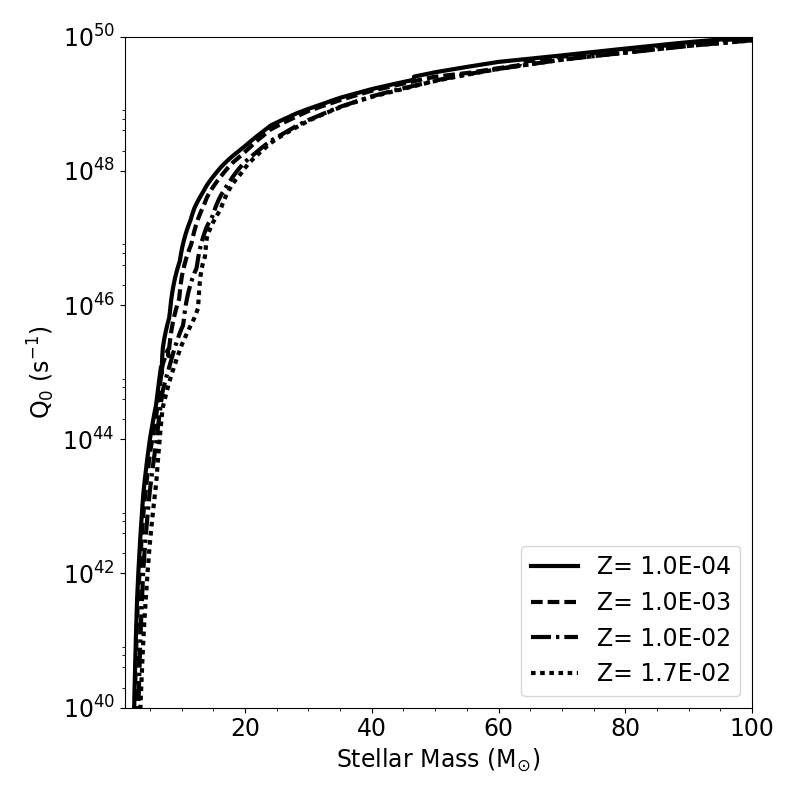
\includegraphics[width=0.4\linewidth]{Q0}
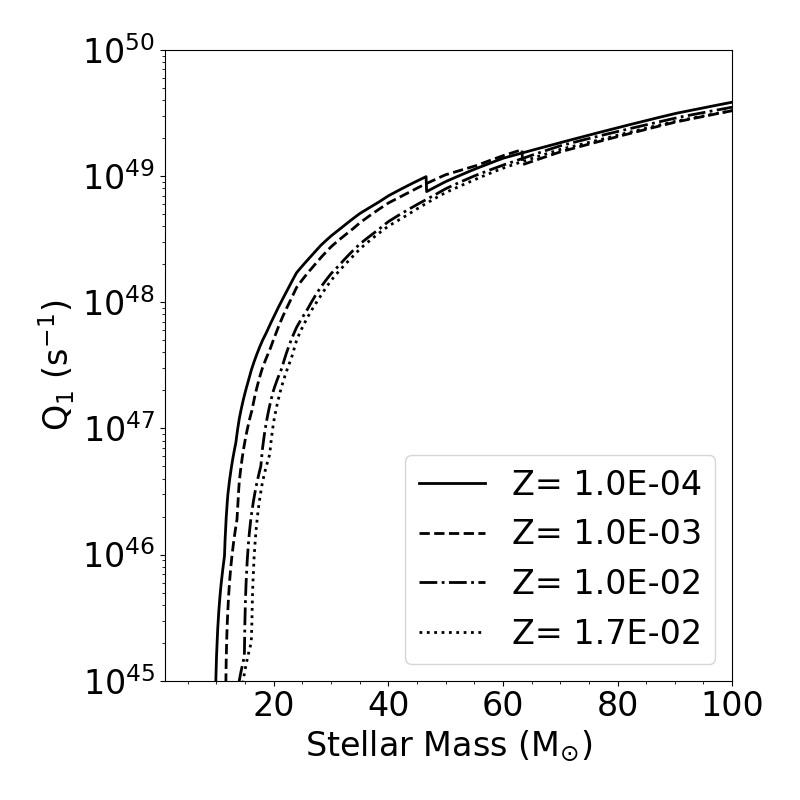
\includegraphics[width=0.4\linewidth]{Q1}
\vspace{0.01cm}
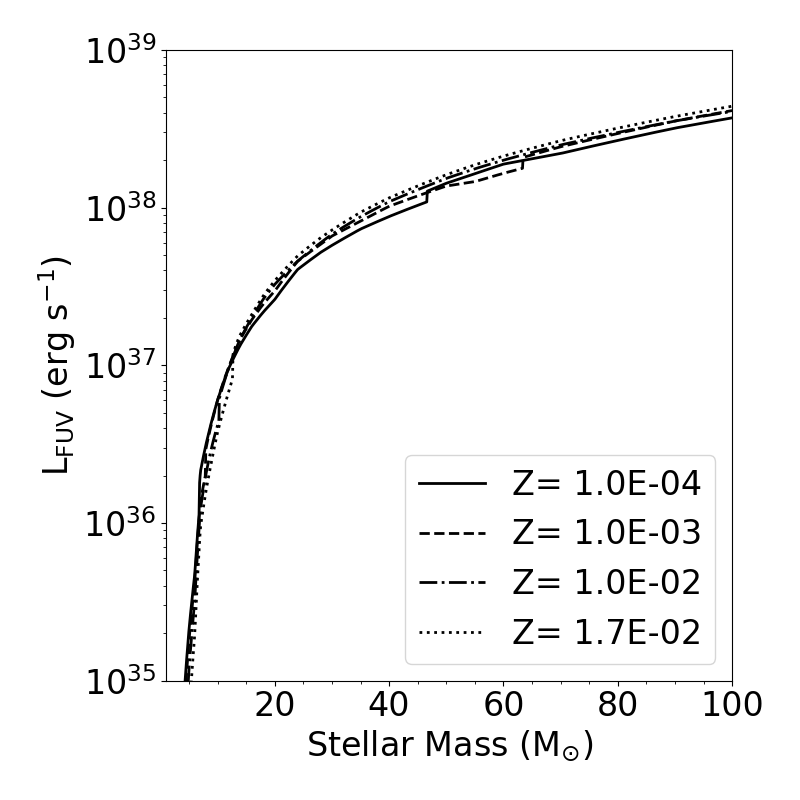
\includegraphics[width=0.4\linewidth]{L_FUV}
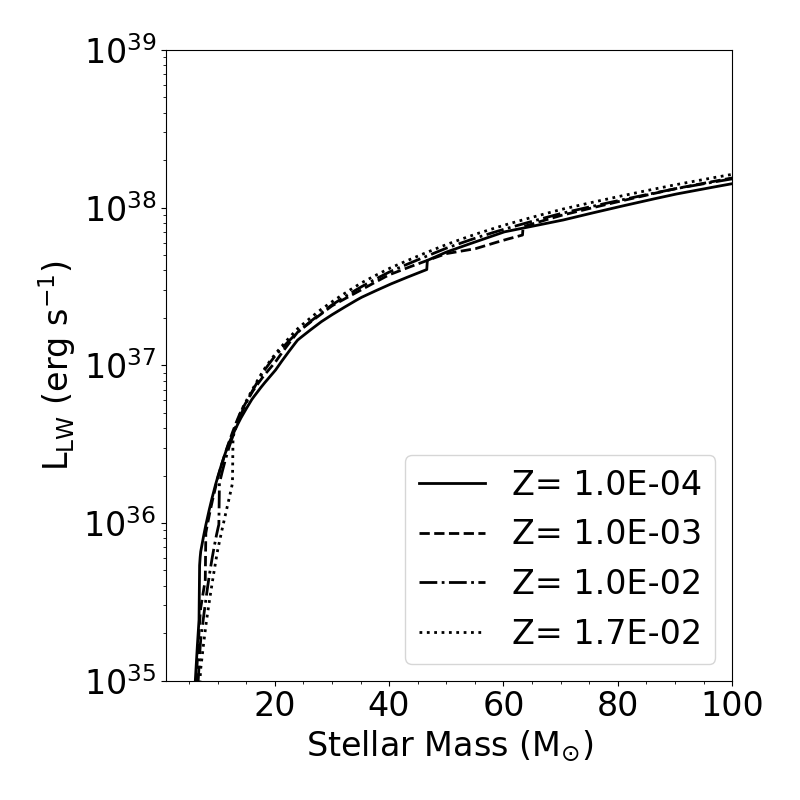
\includegraphics[width=0.4\linewidth]{L_LW}
\vspace{0.01cm}
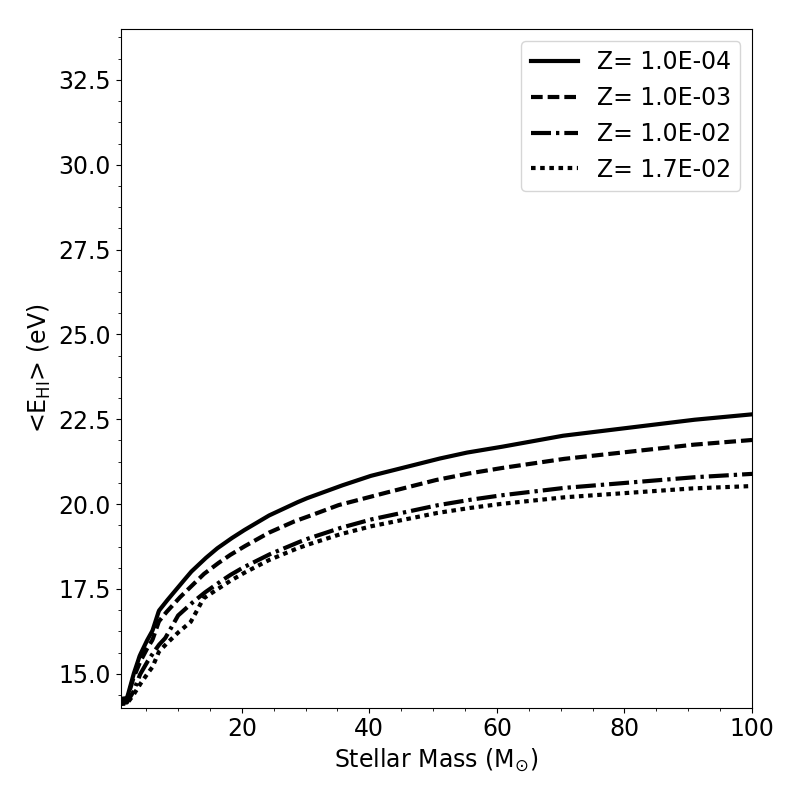
\includegraphics[width=0.4\linewidth]{E0}
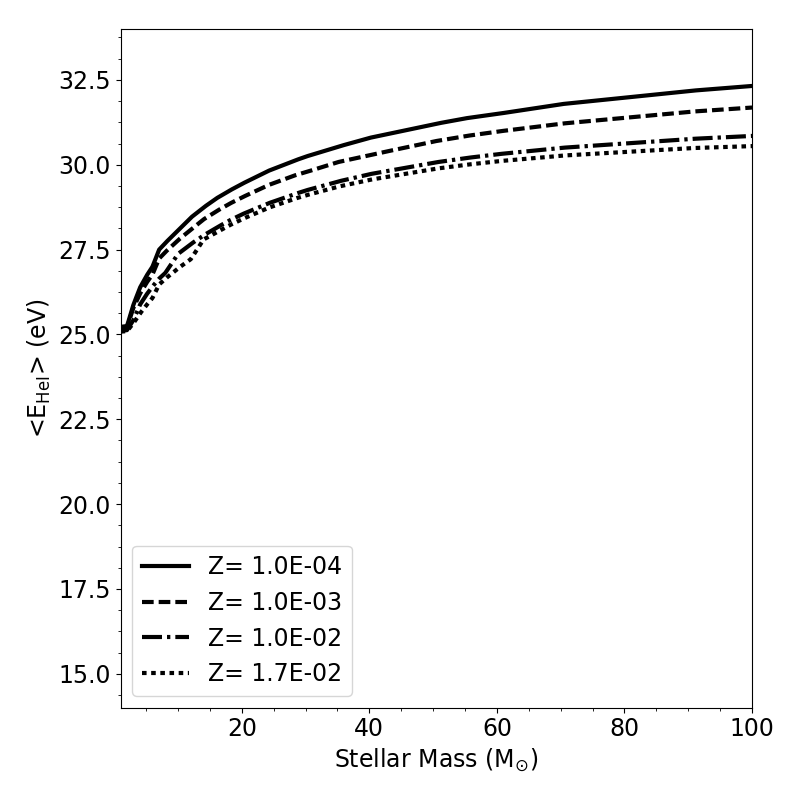
\includegraphics[width=0.4\linewidth]{E1}
\caption{Radiation properties for our model stars. Note, we only track radiation from stars above
8.0 \msun, which dominate over less massive stars, even when accounting for IMF weighting.}
\label{fig:stellar radiation properties}
\end{figure}

\section{Typical Gas Densities in Supernova Injection Regions}
\label{appendix:supernova}

Modeling supernova feedback with the injection of thermal energy alone can lead to rapid over cooling of the injected energy, and a significant underestimate of the effects of supernova feedback. Often, ad hoc solutions to this problem are used in large simulations with coarse resolution, such as momentarily turning off cooling in feedback affected regions or decoupling affected regions from the hydrodynamics for some time. However, physically consistent solutions have been employed \citep[e.g][]{Simpson2016} which inject a mixture of kinetic and thermal energy, whose ratio of kinetic to thermal energy injection depends on resolution and/or local gas density. This over cooling problem improves with higher resolution and lower ISM densities, until eventually pure thermal energy injection is sufficient to resolve each supernova. We take advantage of our high ($\sim$ pc) scale resolution and employ a simple thermal energy injection model for our supernova feedback. Here we demonstrate how well this resolves our supernovae in the comparison simulation presented in this work.

The left panel of Figure ~\ref{fig:supernova histogram} gives the distributions of the max (orange) and average (black) ISM number densities in the supernova injection regions for each supernovae in the simulations presented in this work. As shown, a majority explode in regions at substantially lower densities than the star formation threshold of 200~cm$^{-3}$. For most supernovae, $n_{\rm max} \le 1.0$~cm$^{-3}$, which is due to the substantial pre-supernova feedback included in our simulations. The right panel of Figure ~\ref{fig:supernova histogram} gives the fractional distribution of the calculated radius of pressure driven snowplow ($R_{\rm PDS}$) phase of the Sedov-Taylor expansion, adopting the definitions from \cite{Simpson2016}, given as
\[
R_{\rm PDS} = 
\begin{cases*}
49.3E^{1/4}_{51}n^{-1/2}_{o} & if  Z $\le$ 0.01 \\
18.5E^{2/7}_{51}n^{-3/7}_{o}Z^{-1/7} & if  Z $\ge$ 0.01 \\
\end{cases*}
\]
where $E_{51}$ is the injection energy in units of 10$^{51}$~erg, $n_{o}$ is the number density of the medium, and $Z$ is the metallicity in units of $Z_{o}$. \cite{Simpson2016} found that $R_{\rm PDS} > 4.5 \Delta x$ is needed to resolve the supernova explosion with thermal energy injection alone, assuming uniform density in the injection region. In practice, the injection region is never uniform. We give $R_{\rm PDS}$ assuming uniform density at both the average and maximum number density in the injection region of each supernova. As shown, a majority of supernovae are resolved (to the right of the 4.5$\Delta x$ line), but that up to 10\% are somewhat under-resolved. In general, these are supernova explosions from the most massive (i.e. most prompt) stars. We do not expect that resolving these supernovae will dramatically alter our results, but note that simulations presented in future work will examine lower mass galaxies at higher resolution than those presented here. In those, the supernovae are more resolved, but we note that using our feedback model at resolutions much less than 2 pc will require adopting a different injection mechanism. 

% We use a spherically symmetric thermal dump method of modelling supernova explosions. This is the simplest method possible, but can often result in rapid overcooling of the heated gas, effectively underestimating the effectiveness of supernova feedback. Solutions to this problem can often be ad hoc (e.g. briefly turning off cooling) in low resolution, large cosmological simulations. However, recent work has shown injecting some fraction of this thermal energy directly as kinetic energy or momentum alleviates this issue without sacrificing physical realism. However, it has been shown that simple thermal energy injection is sufficient for parsec scale (or better) resolutions, provided the supernova do not occur in very high density regions; if resolved, thermal injection converges with kinetic energy / momentum injection methods. Resolving these explosions with thermal energy injection alone depends ultimately on the grid resolution, background density and ISM structure, the background cooling/heating physics used, and the size and shape of the injection region. Here, we perform a resolution test of our thermal injection method over four uniform densities (0.1 \ccunit, 1.0 \ccunit, 10.0 \ccunit, and 100.0 \ccunit) for both a 8.0 \msun and 25.0 \msun star, comparing to both the analytic solution and results using kinetic energy injection from \cite{Simpson2015}. These results are presented in Figure~\ref{fig:supernova tests}. We note these are heavily idealized cases. In general in our simulations, pre-SN feedback from stellar winds and radiation will reduce the typical densities within which our supernova explosions occur. In addition, supernova will generally be clustered, meaning each SN will reducing the typical density for each subsequent SN in that region. In Figure~\ref{fig:supernova histogram} we plot a histogram of the typical peak and average gas densities in the 3 cell injection region of each supernova in the XXXX XXXXX simulation. As shown, some of the supernova explode in high density regions around 100 \ccunit and are likely under-resolved, but a majority will be resolved.

\begin{figure}
\centering
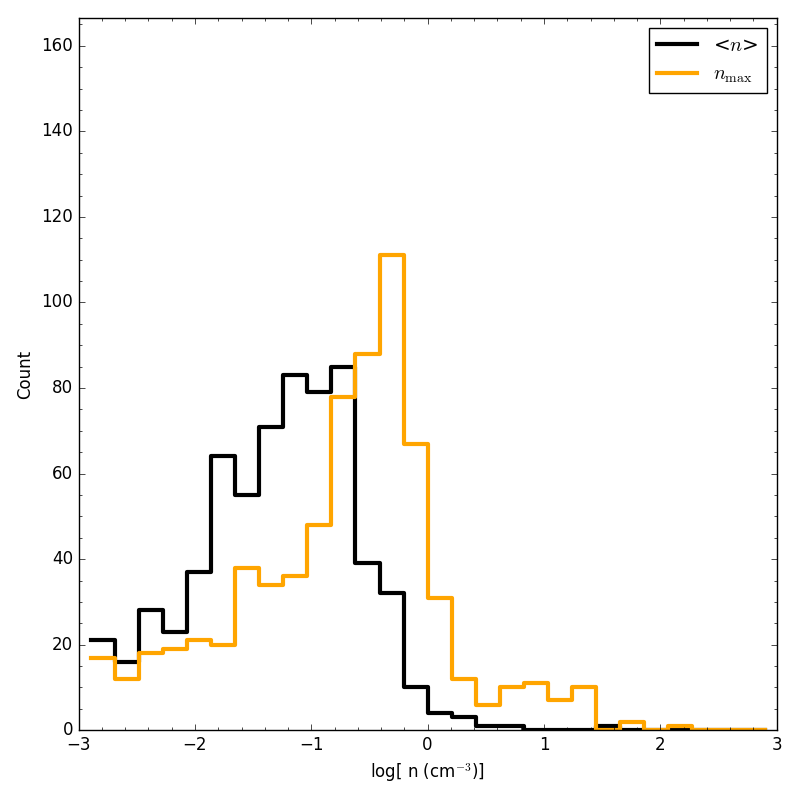
\includegraphics[width=0.4\linewidth]{sn_density_hist}
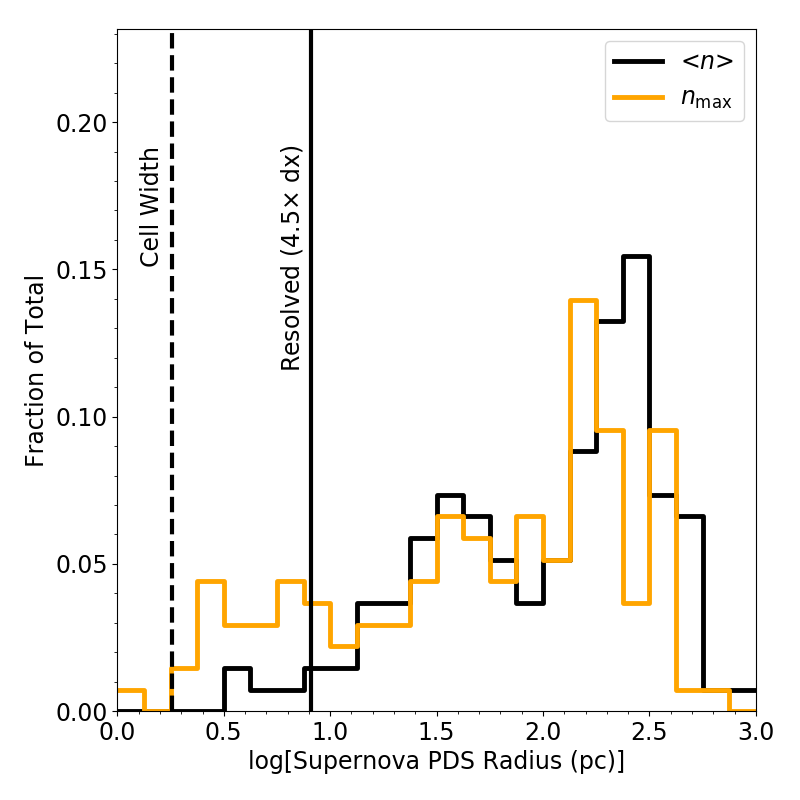
\includegraphics[width=0.4\linewidth]{sn_radius_hist}
\caption{Distribution of peak and average gas densities (left) in the injection region of each of the supernovae from the simulation. On the right, we give the distribution of the radius of the pressure driven snowplow phase for each supernova assuming a uniform medium at either the peak or average density in the injection region. The vertical lines give one and 4.5 cell widths. As shown, a fraction of these SN are certainly under resolved, with R$_{\rm PDS}$ less than a single cell size, but a majority are resolved.}
\label{fig:supernova histogram}
\end{figure}

%\section{Stellar Wind Model}
%\label{appendix:stellar winds}
%
% This is still probably a good idea to do at some point, but save for if/when
% we have a paper using full stellar winds where this matters - AE (Jul. 19 2017)
%
%Discuss wind properties and evolution in a hand full of isolated star runs (don't need to do a resolution study... kinda) and compare to Weaver et. al. 1977 analytic results. Really we won't resolve the winds at high densities, but that is OK... as long as the wind bubbles are > 3*dx (the injection size) we are generally going to be fine... aka as long as the SN explosion goes off in wind bubble gas and not dense ISM that shouldn't be there..

\section{Cooling Rates}
\label{appendix:cooling}
Figure ~\ref{fig:cooling} shows the combined primordial and metal line cooling (dashed) and heating (dotted) rates at three characteristic densities for Z = 0.01 Z$_{\odot}$, closer to the metallicities of our fiducial set of dwarf galaxy simulations (Emerick et. al. in prep). The solid lines give the absolute value of the net cooling rate, which more clearly indicates the regime at low temperatures where heating dominates. The curve as shown includes the z = 0 \cite{HM2012} metagalactic UVB.

\begin{figure}
\centering
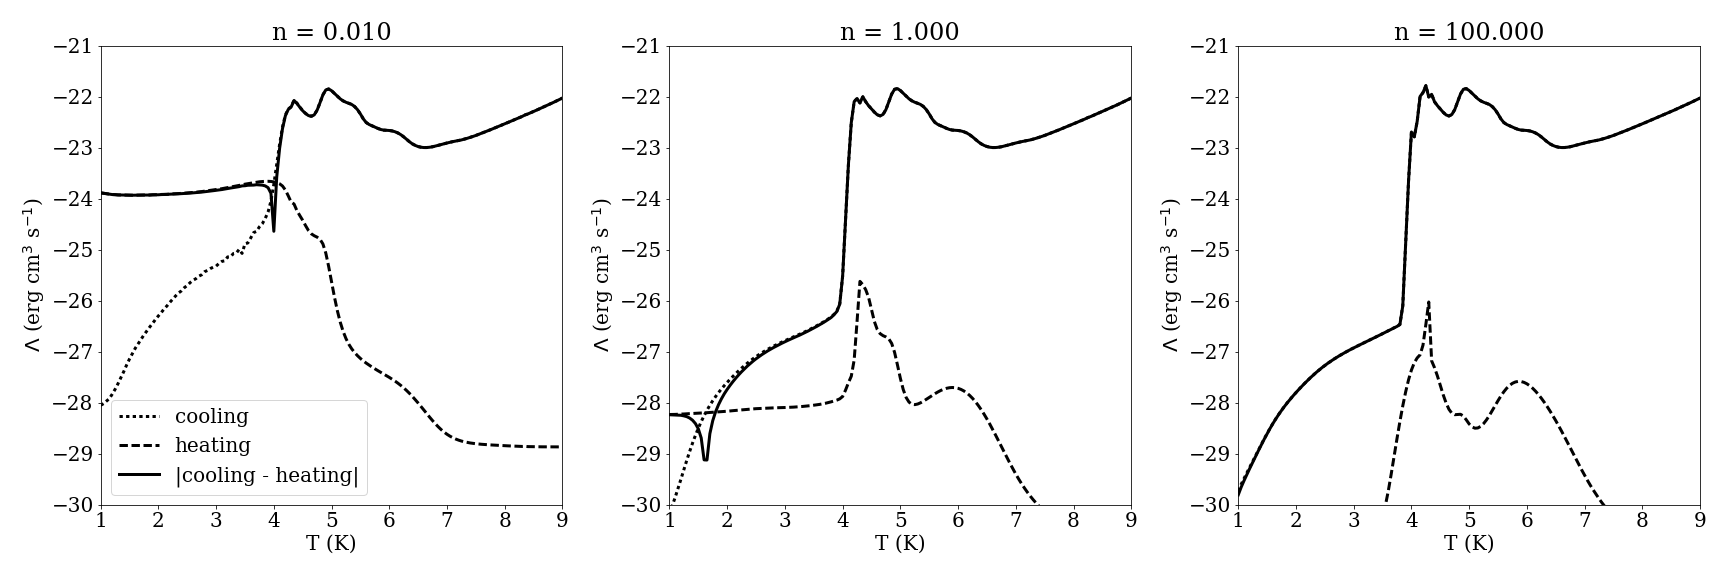
\includegraphics[width=0.95\linewidth]{cooling_curve}
\caption{The total heating and cooling rates extracted from the core of a Jeans-length sized cloud irradiated by a \cite{HM2012} metagalactic background as modeled in \textsc{Cloudy}. The absolute value of the net cooling rate is shown with solid lines.}
\label{fig:cooling}
\end{figure}

We note that this cooling curve shows only an approximation of the local cooling and heating rates used in the simulations for two reasons. First, the primordial cooling and heating rates shown here are those returned by \textsc{Cloudy}, but only the tabulated \textsc{Cloudy} metal line cooling and heating rates are used. The actual primordial heating and cooling rates are calculated self-consistently using the non-equillibrium chemistry solver and the self-shielding approximation from radiative transfer simulations given in \cite{Rahmati2013}. However, given that we remove the optically thin assumption when computing the \textsc{Cloudy} tables, the rates shown should be comparable to the locally varying cooling curve in the simulations. Second, this figure ignores the contributions to the heating rate from the variable interstellar radiation field, namely the stellar contribution to photoelectric heating, heating from LW dissociation, and ionization heating. We describe how we obtain the metal line cooling rates below and quantify the change in using these updated tables. 
%Therefore, the heating rates shown are approximate lower limits to the true heating experienced by any given cell in the simulation.

The cooling curves used in this work correct a significant conceptual inconsistency one may encounter when using tabulated metal line cooling rates in combination with self-shielding approximations. Previous work in \cite{Hu2017} details this inconsistency. In short, adopting tabulated metal cooling rates computed under the assumption of an optically thin UV background overestimates the electron fraction in regimes where self-shielding is important, about $-0.5 \leq \rm{log(n~[cm^{-3}])} < 2$, leading to an overestimation of the metal cooling rates. We demonstrate this effect in Figure~\ref{fig:cooling comparison}, which gives |cooling - heating| for our full model at $Z = 0.1~Z_{\odot}$ (black) as compared to a model using the optically thin metal line cooling rates (orange) at a range of densities. The effect is most significant at moderate densities, where the net cooling rate can be an order of magnitude higher. In low temperature regions, this can significantly shift the inferred equilibrium temperature.

The cooling curve shown in Figure~\ref{fig:cooling} avoids this discrepancy using re-computed metal line cooling tables. We have made these tables publicly available in the main distribution of \texttt{Grackle}. For densities where self-shielding is important, we computed \texttt{Cloudy} models of 1D clouds at each temperature and density pair with a physical size corresponding to the Jeans length. In cases where the Jeans length is very large, we limit the size to 100 pc, a reasonable approximation for the maximum size of a self-gravitating cloud. We then adopt the metal line cooling rates obtained from the center of these clouds, whose outside is exposed to the UVB. These models were computed with a modified version of the \texttt{CIAOLoop}\footnote{https://bitbucket.org/brittonsmith/cloudy\_cooling\_tools (our version: https://github.com/aemerick/cloudy\_tools)} code used in \citet{2008MNRAS.385.1443S}. In computing these tables we had to include the CR ionization that dominates in optically thick clouds. Without this effect, \texttt{Cloudy} becomes unstable in entirely neutral regions. We adopted a CR ionization rate of 10\% the MW value, though we note varying this from 1\% to 100\% the MW value did not have an effect on the extracted metal line cooling rates. 

\begin{figure}
\centering
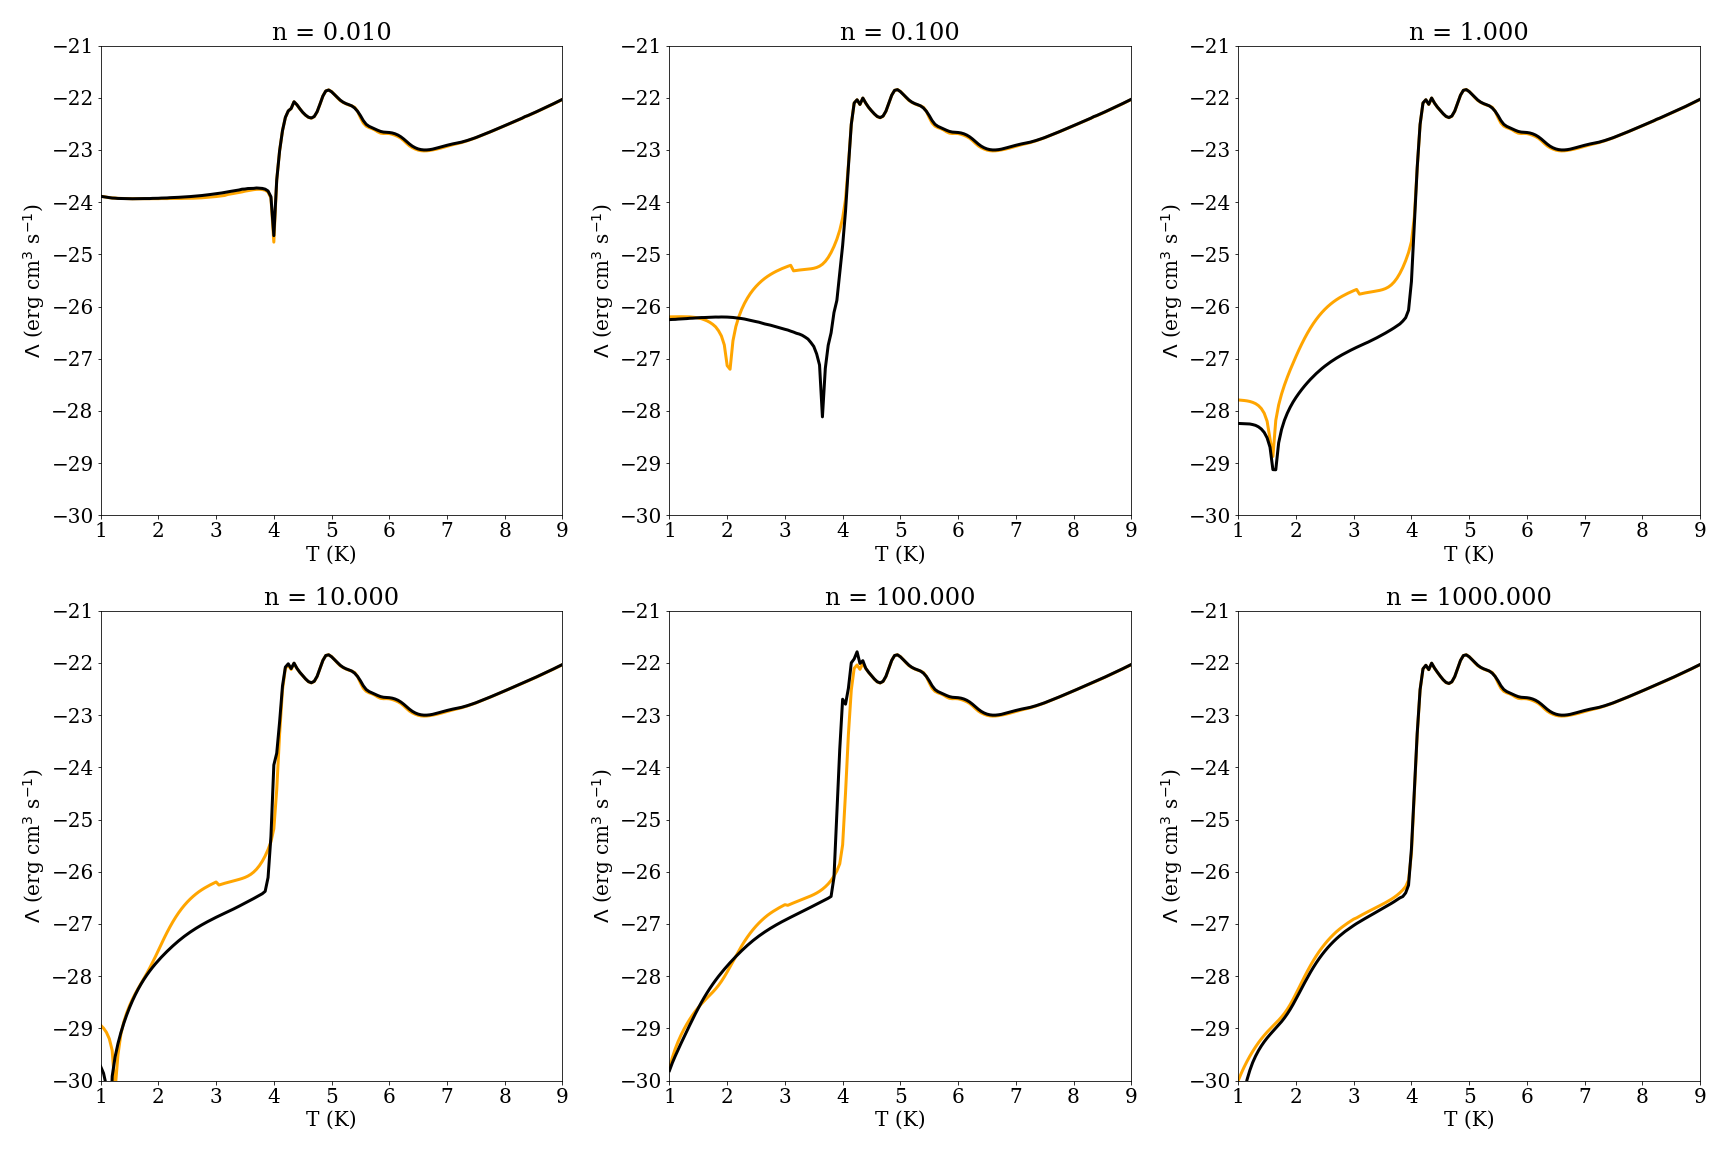
\includegraphics[width=0.95\linewidth]{cooling_model_comparison}
\caption{The absolute value of the net cooling rate (|cooling - heating|) in two models that account for self-shielding of primordial gas against a metagalactic UV background. Our model (black) uses self-consistent metal line cooling rates, and is compared to an incorrect model (orange) that adopts the un-corrected (i.e. optically thin) metal line cooling rates.}
\label{fig:cooling comparison}
\end{figure}

%\section{Pre-SN Feedback with and without radiation}

%\section{Code}
%(likely just do this as a short blurb in acknowledgements)

%A one-zone chemical evolution and feedback model was constructed to provide rapid testing and examination of the feedback and yield properties of each of our stars in our model. This code is publically available at https://github.com/aemerick/onez. In the simplest case, one can generate a series of star particles and examine their resulting properties, including wind and supernova yields, as a function of mass and metallicity. Included also are more complicated examples of running the full one-zone model. Support currently only exists for running in a non-cosmological mode with a constant star formation rate. In addition, this one-zone model uses star-by-star modelling and becomes extremely inefficient at large particle counts. Future develop will better optimize this code, allow for variable input or evolving star formation rates, cosmological evolution, and parallelism. 






%\appendix
%\section{appendix section}

\end{document}
